% \documentclass{ijsra}
\def\IJSRAidentifier{\currfilebase} %<---- don’t change this!
\def\submission{}%YYYY-MM-DD
\def\acceptance{}%YYYY-MM-DD
%-------Title | Email | Keywords | Abstract-------------
\def\shorttitle{The Green and White Grocery}
\def\maintitle{The Green and White Grocery: Change and continuity on Austin’s East Side}
\def\cmail{zl1009@txstate.edu}
\def\keywords{Historical Archaeology, Vernacular Architecture, Mexican-American Studies, Chicano History, \emph{botánica}, minority businesses, grocery store, religion}
%\def\keywordname{}%<--- redefine the name “Keywords“ in needed language
\def\abstract{As more historic structures in East Austin, Texas are lost to the forces of gentrification, this paper demonstrates the importance to the Austin Mexican-American community of one such structure listed in a recent survey but not yet identified for historic preservation. The Green and White Grocery is an American Craftsman-style grocery store/botánica in Austin, Texas dating to the late 1930s or early 1940s. It is owned by John Lopez Cazares, descendant of the original owners Noberto and Susie Lopez. Basic surveying of the structure’s elevation and floor plan, documentary research, and oral interviews with Cazares reveal the business’s impact on the community, the reasons for certain design and aesthetic choices, and how the structure went from being a traditional grocery store to a store selling personal religious iconography. Little archaeological work on Mexican-American grocery stores exists; this paper also contextualizes the store compared to similar African-American stores that have been researched. While it is important not to assume decisions made by Noberto and Susie Lopez apply to the broader Mexican-American community, I hope to provide ideas for further comparative research.}
%--------Author’s names------------
\def\authorone{Zach Lindsey}
%-------Biographical information-------------
\def\bioone{Zach Lindsey is interested in the way people use language and iconography to educate each other and spread ideological beliefs, especially in the Mesoamerican region. He is a student of anthropology, a former journalist, and a soon-to-be dad. This paper was written for the Archaeology of Standing Structures course during a Postgraduate Certificate at the University of Leicester (UK).}
%------University/Institution--------------
\def\affilone{Master’s student, Texas State University}

\begin{filecontents}{\IJSRAidentifier.bib}
@unpublished{anon,
	author = {Anonymous},
	month = {7},
	note = {Photograph},
	title = {Green and White Grocery Store},
	year = {1958},
	url = {texashistory.unt.edu/ark:/67531/metapth531415/},
	comment = {University of North Texas Libraries},
}

@book{anzaldua,
	author    = "Anzaldua, G.",
	title     = "Borderlands/La Frontera: The New Mestiza",
	publisher = "Aunt Lute",
	year      = "2012",
	address   = "San Francisco"
}

@incollection{ashmore,
	address = {Oxford},
	author = {Ashmore, W.},
	booktitle = {Mesoamerican Archaeology},
	editor = {J. Hendon and R. Joyce},
	pages = {169-191},
	publisher = {Blackwell},
	title = {Classic Maya Landscapes and Settlement},
	year = {2004},
}

@article{barragan,
	author = {Barragan, J.},
	publisher = {Austin American-Statesman},
	title = {Quietly, lawsuit over Jumpolin pinata store demolition is resolved},
	year = {2015},
	url = {http://www.statesman.com/news/local/quietly-lawsuit-over-jumpolin-pinata-store-demolition-resolved/wscvBWvCw7Spi4pyXsT9cP},
	comment = {Accessed 05/12/2017},
}

@book{becker,
	author = {Becker, T., J. Boisvenue and S. Garcia},
	note = {Video},
	publisher = {The East Austin Project},
	title = {The Green and White},
	year = {2003},
	url = {https://youtu.be/a77OV42ISHY},
}

@article{campion,
	author = {Campion, G.},
	journal = {Antiquity},
	pages = {847-860},
	title = {People, Process and the Poverty-Pew: a functional analysis of mundane buildings in the Nottinghamshire framework-knitting industry.},
	volume = {70},
	year = {1996},
}

@article{delgado,
	author = {Delgado, M. and D. Humm-Delgado},
	journal = {Social Work},
	number = {1},
	pages = {83-89},
	title = {Natural Support Systems: Source of Strength in Hispanic Communities},
	volume = {27},
	year = {1982},
}

@article{fisch,
	author = {Fisch, S.},
	journal = {The Milbank Memorial Fund Quarterly},
	number = {3},
	pages = {377-388},
	title = {Botanicas and Spiritualism in a Metropolis},
	volume = {46},
	year = {1968},
}

@book{frampton,
	address = {New York},
	author = {Frampton, K.},
	publisher = {Oxford},
	title = {Modern Architecture: A Critical History},
	year = {1982},
}

@article{gandara,
	author = {Gandara, R.},
	publisher = {Austin American-Statesman},
	title = {Longtime Green and White Grocery Owner Remembered for Kindness to All},
	year = {2012},
	url = {http://www.statesman.com/news/local/longtime-green-white-grocery-owner-remembered-for-kindness-all/HavYksN29sukmzss1rKQtM/},
	comment = {Accessed 05/15/2017},
}

@book{glassie,
	address = {Bloomington},
	author = {Glassie, H.},
	publisher = {Indiana University},
	title = {Vernacular Architecture},
	year = {2000},
}

@article{googlemaps,
	author = {Google Maps},
	title = {Google Maps location for 1201 E 7th St. Austin, TX},
	year = {2017},
	url = {https://www.google.com/maps/place/Green+and+White+Grocery/@30.2649964,-97.7301178,20z/data=!4m5!3m4!1s0x0:0x63bde337444e6a51!8m2!3d30.2650983!4d-97.7300119},
	comment = {Accessed 05/11/2017},
}

@book{hardy,
	address = {TX},
	author = {Hardy, Heck and Moore, Inc},
	publisher = {Hardy, Heck and Moore, Inc},
	title = {City of Austin Historic Resources Survey},
	volume = {IV},
	year = {2016},
}
%how do we format this reference author (company name)

@article{hernandez,
	author = {Hernandez-Ehrisman, L.},
	publisher = {The End of Austin},
	title = {Breakfast Taco Wars: Race, History, and Food in Austin and San Antonio},
	year = {2016},
	url = {https://endofaustin.com/2016/09/22/breakfast-taco-wars-race-history-and-food-in-austin-and-san-antonio/},
	comment = {Accessed 05/13/2017},
}

@incollection{joyce,
	address = {Oxford},
	author = {Joyce, R.},
	booktitle = {Mesoamerican Archaeology},
	editor = {J. Hendon and R. Joyce},
	pages = {1-42},
	publisher = {Blackwell},
	title = {Mesoamerica: A Working Model for Archaeology},
	year = {2004},
}

@book{kerr,
	author = {Kerr, B.},
	publisher = {Austin Chamber},
	title = {Greater Austin Profile: Population},
	year = {2016},
	url = {https://www.austinchamber.com/upload/files/ed/population.XLS},
	comment = {Accessed 04/30/2017},
}

@article{kreneck,
	author = {Kreneck, T.},
	journal = {The American Archivist},
	number = {3},
	pages = {272-276, 278-285},
	title = {Documenting a Mexican American Community: The Houston Example},
	volume = {48},
}

@book{lane,
	author = {Lane, R.},
	publisher = {Historic England},
	title = {Understanding Historic Buildings: A Guide to Good Recording Practice},
	year = {2016},
}

@book{lepe,
	author = {Lepe, E.},
	publisher = {The East Austin Project},
	title = {The History of the Green \& White Store},
	year = {2002},
	url = {https://youtu.be/FKsKnojVWHo},
}

@book{linne,
	address = {Tuscaloosa},
	author = {Linne, S.},
	publisher = {University of Alabama},
	title = {Archaeological Researches at Teotihuacan, Mexico},
	year = {2003},
}

@book{miller,
	author = {Miller Blue Print},
	title = {Austin Texas Street Guide},
	year = {1934},
	url = {https://www.lib.utexas.edu/maps/texas/austin-redlining-large-1935.jpg},
	comment = {Accessed 05/17/2017},
}

@book{moreland,
	address = {London},
	author = {Moreland, J.},
	publisher = {Duckworth},
	title = {Archaeology and Text},
	year = {2001},
}

@BOOK {morner,
	author    = "Mörner, M.",
	title     = "Race Mixture in the History of Latin America",
	publisher = "Little, Brown \& Company",
	year      = "1967",
	address   = "Boston"
}

@article{mullins,
	author = {Mullins, P.},
	journal = {Historical Archaeology},
	number = {1},
	pages = {88-96},
	title = {Marketing in a Multicultural Neighborhood: An Archaeology of Corner Stores in the Urban Midwest},
	volume = {42},
	year = {2008},
}

@book{pluciennik,
	address = {Leicester},
	author = {Pluciennik, M. and C. Newman and M. Godfrey},
	publisher = {University of Leicester},
	title = {The Archaeology of Standing Buildings},
	year = {2015},
}%this source doesn't seem to exist? need to check with author

@article{romberg1998,
	author = {Romberg, R.},
	journal = {Journal of Folklore Research},
	number = {1},
	pages = {69-82},
	title = {Whose Spirits Are They? The Political Economy of Syncretism and Authenticity},
	volume = {35},
	year = {1998},
}

@article{romberg2005,
	author = {Romberg, R.},
	journal = {NWIG: New West Indian Guide/Nieuwe West-Indische Gids},
	pages = {175-218},
	title = {Ritual Piracy of Creolization with an Attitude},
	volume = {79},
	year = {2005},
}

@book{robinson,
	author = {Robinson, W.},
	publisher = {Handbook of Texas Online},
	title = {Architecture},
	year = {2010},
	url = {http://www.tshaonline.org/handbook/online/articles/cmask},
	comment = {Accessed 04/29/2017},
}

@book{sanborn,
	address = {New York},
	author = {Sanborn Map Company},
	publisher = {Sanborn},
	title = {'Austin 1935 Key Map.' New York: Sanborn},
	year = {1935},
	url = {https://texashistory.unt.edu/ark:67531/metapth575205},
	comment = {Accessed 5/23/2017},
}

@book{swallow,
	address = {Dorset},
	author = {Swallow, P. and R. Dallas and S. Jackson and D. Watt},
	publisher = {Donhead},
	title = {Measurement and Recording of Historic Buildings},
	year = {2008},
}%reference not used

@unpublished{tcad,
	author = {TCAD},
	note = {Search query: Green \& White Grocery 0205070101},
	title = {Travis Central Appraisal District property search},
	year = {2017},
	url = {https://propaccess.traviscad.org/clientdb/?cid=1},
	comment = {Accessed 05/10/2017},
}

\end{filecontents}
\IJSRAopening%<---- don’t change this!
%-------
\lettrine{T}{he} population of Austin, Texas grew from \num{1.2} million in 2000 to more than \num{2} million in 2015, and has grown by \num{37} percent in the last five years alone (\cite{kerr}). The resulting demographic pressures have changed the city's cultural landscape. One of the front lines in the city's gentrification is East Austin, a region usually defined as east of Interstate-35 and north of the Colorado River (\cite{hernandez}).

East Austin is historically important for minority, especially Latino, residents of the city (\cite{hernandez}). Texas was once part of Mexico, and Mexican-American cultural influence in Austin includes everything from an obsession with breakfast tacos (\cite{hernandez}) to \emph{botánicas} 
-- small stores selling localized religious paraphernalia such as incense, Catholic votive-style candles, and herbs --
and other representations of the complex belief system developed in Mexico and the southern United States (\cite{kreneck}).

Lack of resources and interest has left historic structures in the area relatively unprotected. But the city government has not completely forgotten the importance of the region. A 2016 survey by \emph{Hardy, Heck, Moore, Inc.} lists \num{345} structures that surveyors believe could be considered for local historic recognition, but constraints of the survey limit the level of detail provided for specific individual structures. The \emph{Hardy, Heck, Moore, Inc.} survey includes a two-page report on each structure and two standard (i.e., non-rectified or otherwise edited) photographs. This might be considered the most basic level of surveying according to \textcite[25]{lane} or \textcite[370]{pluciennik}. 
While limited, the reports provide strong foundations for further research, such as approximate dates of building ownership pulled from city records. However, for a business in a minority community, a cursory summary may miss important details. 
An example at the Green and White Grocery (\cref{fig:Lindsey_Figure_01}, \cref{fig:Lindsey_Figure_02}, and \cref{fig:Lindsey_Figure_03}) is a conflict over dates: the owner commented during an interview that the business dates to the 1930s, but city directories do not have an address for that property before 1940 
\parencite[75-76]{hardy}.

%FIGURE 01: The Grocery
\begin{figure}[!p]
\begin{minipage}[t]{.49\linewidth}
	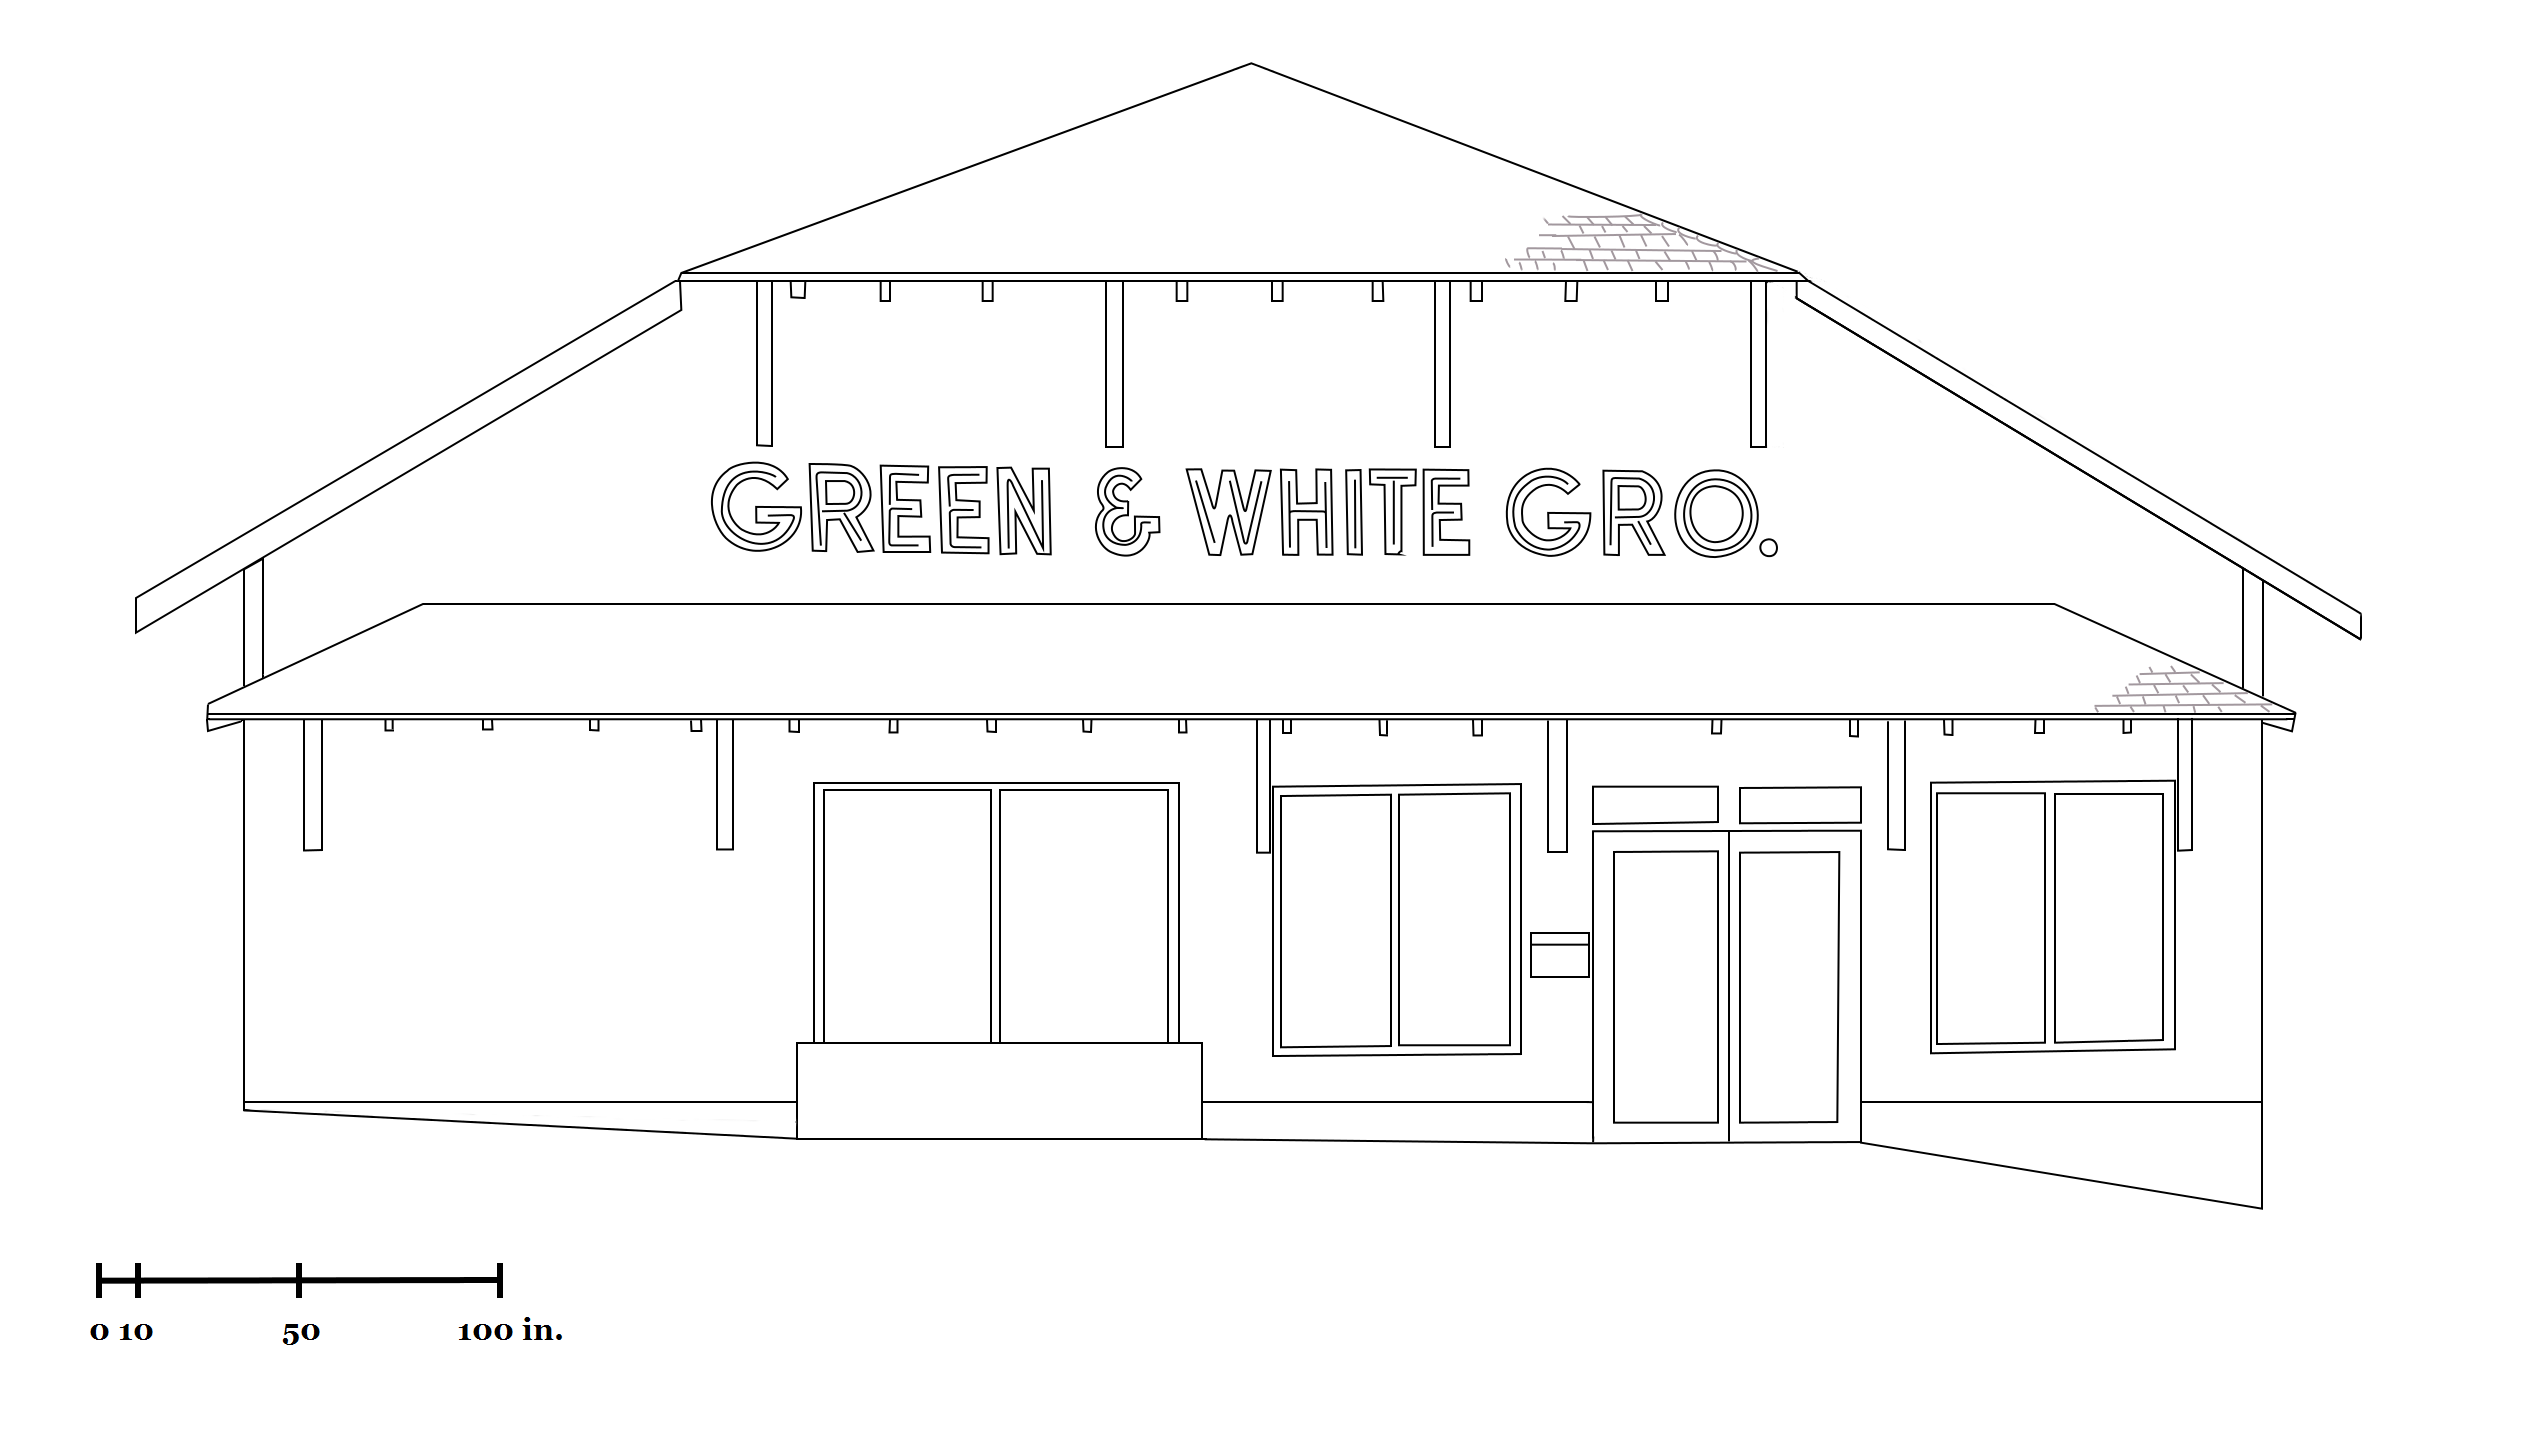
\includegraphics[width=\linewidth]{Lindsey_Figure_01}
	\caption{The Green and White Grocery at 1201 E. \nth{7} St. on the corner of Waller and E. \nth{7} 
(Property ID 192881, Geographic ID 0205070101) 
in Austin, TX. Northern elevation\\
		{\normalfont\scriptsize \copyright\
			\shortauthor, illustration
	}}
	\label{fig:Lindsey_Figure_01}
\end{minipage}
\hfill
%FIGURE 02: Floor plan
\begin{minipage}[t]{.49\linewidth}
	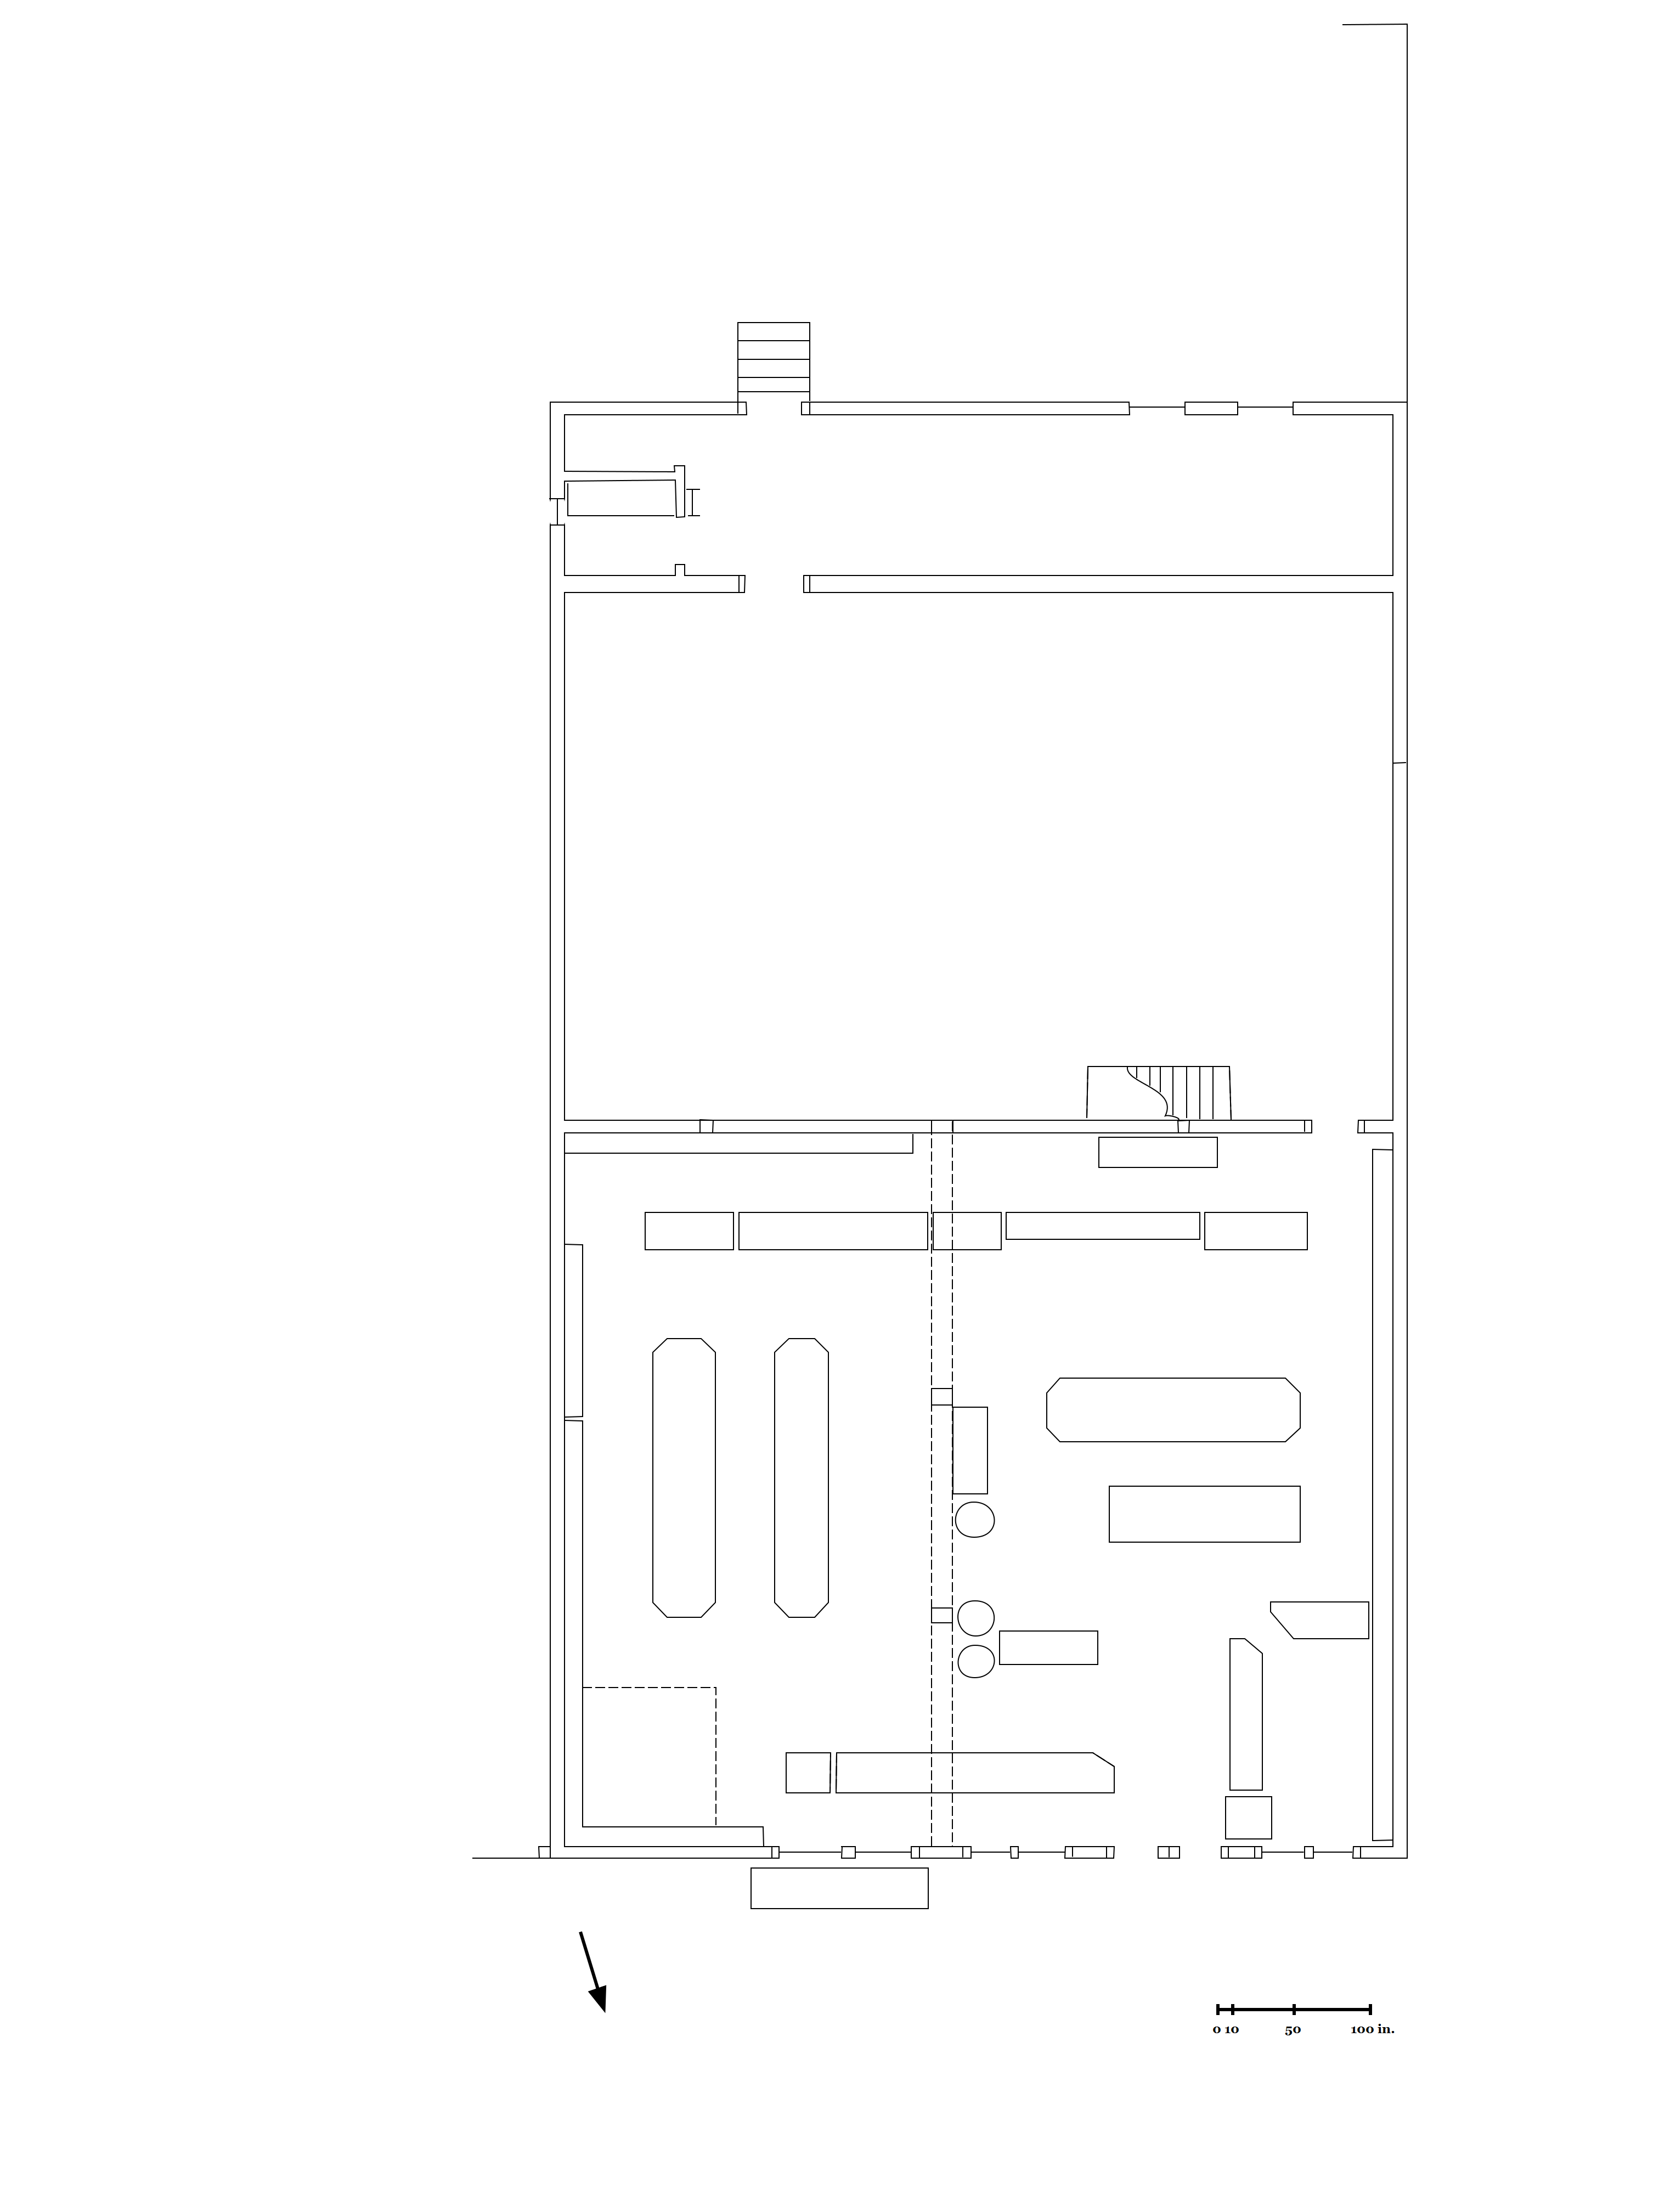
\includegraphics[width=\linewidth]{Lindsey_Figure_02}
	\caption{Floor plan of the Green and White Grocery\\
		{\normalfont\scriptsize \copyright\
			\shortauthor
	}}
	\label{fig:Lindsey_Figure_02}
\end{minipage}
\end{figure}

A larger detail overlooked by the survey is the fact that the Green and White Grocery is not a grocery store at all. Like many buildings, it has evolved since its opening. It began as a taco stand and became a traditional Mexican-American grocery store selling tamales, dry goods such as beans and rice, salsas and hot sauces, and ice out of an ice box, as well as some religious paraphernalia. At some point in its early history, its owners probably built a rear extension and eventually sealed the opening for the ice box, but in general, I believe the outer structure has changed little. Yet as new family members took over, it lost the food and became a botánica. The change may seem radical, but the continuity of family ownership and the family’s role in the Mexican-American community mean that the building itself has changed perhaps less than an outsider might expect.

%FIGURE 03: Map of area
\begin{figure}[!p]
	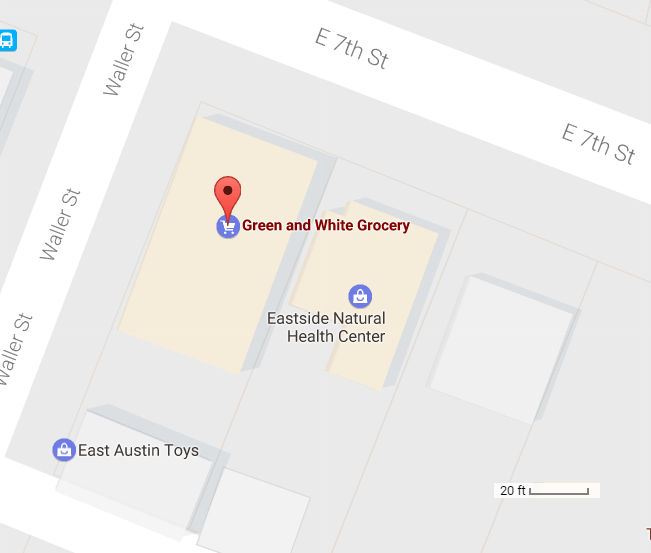
\includegraphics[width=.7\linewidth]{Lindsey_Figure_03}
	\caption{A 2017 map of the area around the Green and White Grocery created using Google Maps \\
		{\normalfont\scriptsize \copyright\ \textcite{googlemaps}
	}}
	\label{fig:Lindsey_Figure_03}
\end{figure}

The façade of the Green and White Grocery is similar to the original structure and current owner John Lopez Cazares, who is the grandson of original owners Noberto and Susie Lopez, claims to have left most floor shelving as it was, making it ideal for studies of the design choices of past and current owners. These sorts of studies are the heart of vernacular architecture as defined by \textcite{glassie}. Vernacular architecture focuses on the history of quotidian structures as a way of making statements about the society in which they were built. In this field, design choices represent culturally-influenced decisions, and a design choice can thus tell us about the culture in which the designers lived.

Little archaeological research exists on Mexican-American grocery stores, despite their importance in communities and the potential for insights about diet and lifestyle choices (\cite[279]{kreneck}). However, research exists on similar African-American grocery stores in urban areas, such as that by \textcite{mullins}. This research allows me to make certain comparative statements, but they are limited by the broad differences between Mexican-American and African-American communities. While these differences could make an entire research project in their own right, for the purposes of this paper, access to culture is perhaps the biggest difference. Mexican-Americans face discrimination in Texas, but they are able to interact with Mexican traditions. However, for African-Americans, “the slavery system imposed a filter which very few African traditions were able to penetrate” (\cite[122]{morner}). This can be seen by the scarcity of African-style goods found by \textcite{mullins}. In some cases, the only characteristic that the Green and White Grocery and the spaces examined by Mullins share is that they are minority-owned businesses.
Botánicas and the personalized Spiritist beliefs of their patrons have been investigated for decades in U.S. scholarship (e.g., \cites{delgado}{fisch}{romberg2005}). Unsurprisingly, this scholarship becomes less problematic over time, but little of it addresses actual spatial considerations of botánicas or the buildings that they occupy. A single building cannot be considered a portrait of a community. Due to lack of research in the surrounding area it is impossible to say how similar the Green and White Grocery is to other grocery stores or botánicas. Still, I hope this study can serve as a starting point both for preservation of the Green and White Grocery and for broader comments on the history of Mexican-American owned businesses.

\IJSRAsection{What we think we know}

Before we take a tour of the building, it is important to acknowledge the difficulty of documentary research when it comes to minority-owned businesses. Documents are artifacts of their time, and should be weighed beside the material culture actually found at sites (\cite{moreland}). This is true in the case of the Green and White Grocery, where the Travis Central Appraisal District lists the structure as having been built in 1920 (\cite{tcad}), but neither Cazares himself nor \textcite[75-76]{hardy} agree with this statement. Cazares's grandfather may have owned the property by 1920, although Cazares suggests that his grandfather bought it at a later date, probably 1936. The idea of a later date for the building itself is supported by its absence from a 1921 Sanborn fire insurance map according to \textcite[75-76]{hardy}. Sanborn maps can be powerful resources for historic research, as they typically include detailed lot sizes of buildings assessed for liability purposes. These maps show the addition of new lots over time. But Sanborn maps are poor records regarding East Austin, and their most closely dated map from 1935 \parencite{sanborn} does not include East Austin at all.

However, a 1934 map suggests why Sanborn might not have been so concerned with East Austin. The 1934 map describes which Austin neighborhoods are “best” and which are “hazardous” (\cite{miller}). The region of the city with the most “hazardous” areas was East Austin. As mentioned, East Austin was a low-income area with a large minority population (\cite{hernandez}). The property where the Green and White Grocery would stand was in this supposed “hazardous” area of East Austin. Telling as this is about Austin's imaginings of its minority population, the 1934 map also does not show individual lots, only neighborhood groups.

%FIGURE 04: Historic photo of the structure
\begin{figure}[!tb]
\begin{minipage}[t]{.49\linewidth}
	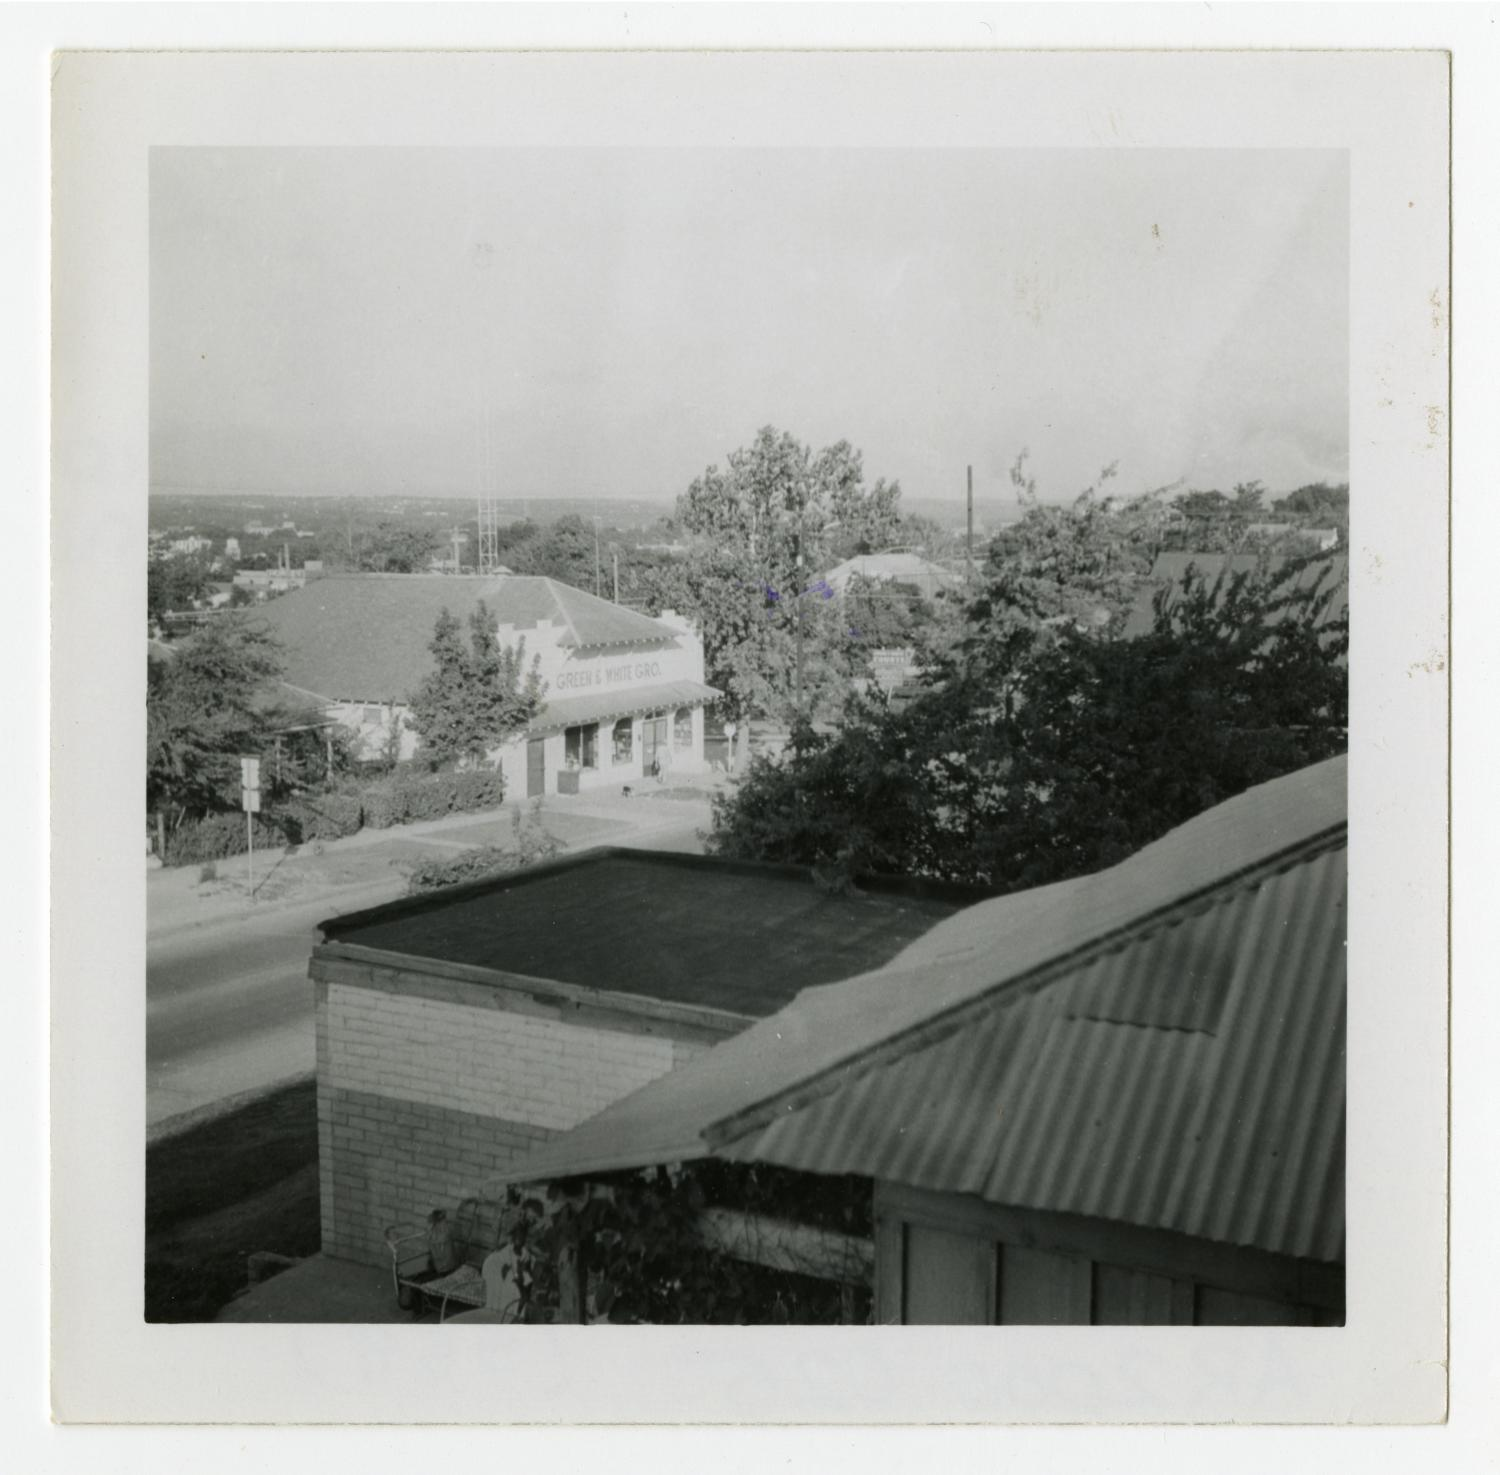
\includegraphics[width=\linewidth]{Lindsey_Figure_04}
	\caption{Historic photo of the structure\\
		{\normalfont\scriptsize %\copyright\
		Source:  \textcite{anon}.
	%\shortauthor
	}}
	\label{fig:Lindsey_Figure_04}
\end{minipage}\hfill
\begin{minipage}[t]{.49\linewidth}
%FIGURE 05: Northeastern approach
	\includegraphics[width=\linewidth]{Lindsey_Figure_05}
	\caption{Northeastern approach\\
		{\normalfont\scriptsize \copyright\
			\shortauthor
	}}
	\label{fig:Lindsey_Figure_05}
\end{minipage}
\end{figure}

A photograph from 1958 though provides documentary evidence of the building's facade (\cite{anon}, \cref{fig:Lindsey_Figure_04}), which has been more or less maintained in the intervening years. While not a formally-recognized historic building, the Green and White Grocery has been recognized in the 21st century by local groups for its role in East Austin history. Two examples of this are available on YouTube through the East Austin Project (\cites{becker}{lepe}). These videos include footage of the facade and interior, supporting Cazares's comments that he has not made major changes, at least not in the last two decades.

\IJSRAsection{A tour of the Green and White Grocery}

If you expect to grab some eggs and milk at the Green and White Grocery, your first sign that you may not get what you came for would not be the building itself, nor the logo which looks little different than it did in 1958 (\cref{fig:Lindsey_Figure_05}). The Green and White Grocery is an American Craftsman structure (\cite[75-76]{hardy}), a style derived from the Arts and Crafts movement which is typified by rustic or naturalistic objects designed to suggest quality workmanship (\cite[42-56]{frampton}). But in Texas, American Craftsman specifically describes a type of one-story building which was popular in the early 1900s, probably inspired by Californian architects Charles and Henry Greene (\cite{robinson}).



The Green and White Grocery's double eaves and roof slope suggest this style, but most American Craftsman structures were houses, not stores (\cite{robinson}). You will not mistake the Green and White Grocery for a house: between its double eaves, capital letters spell out the store's name, stylized as “GREEN \& WHITE GRO” (\cref{fig:Lindsey_Figure_06}). The large glass windows and double doors are also signatures of a commercial operation. But from the outside, you might mistake the Green and White Grocery for a traditional grocery store.

%FIGURE 06: Floor plan
\begin{figure}[!tb]
	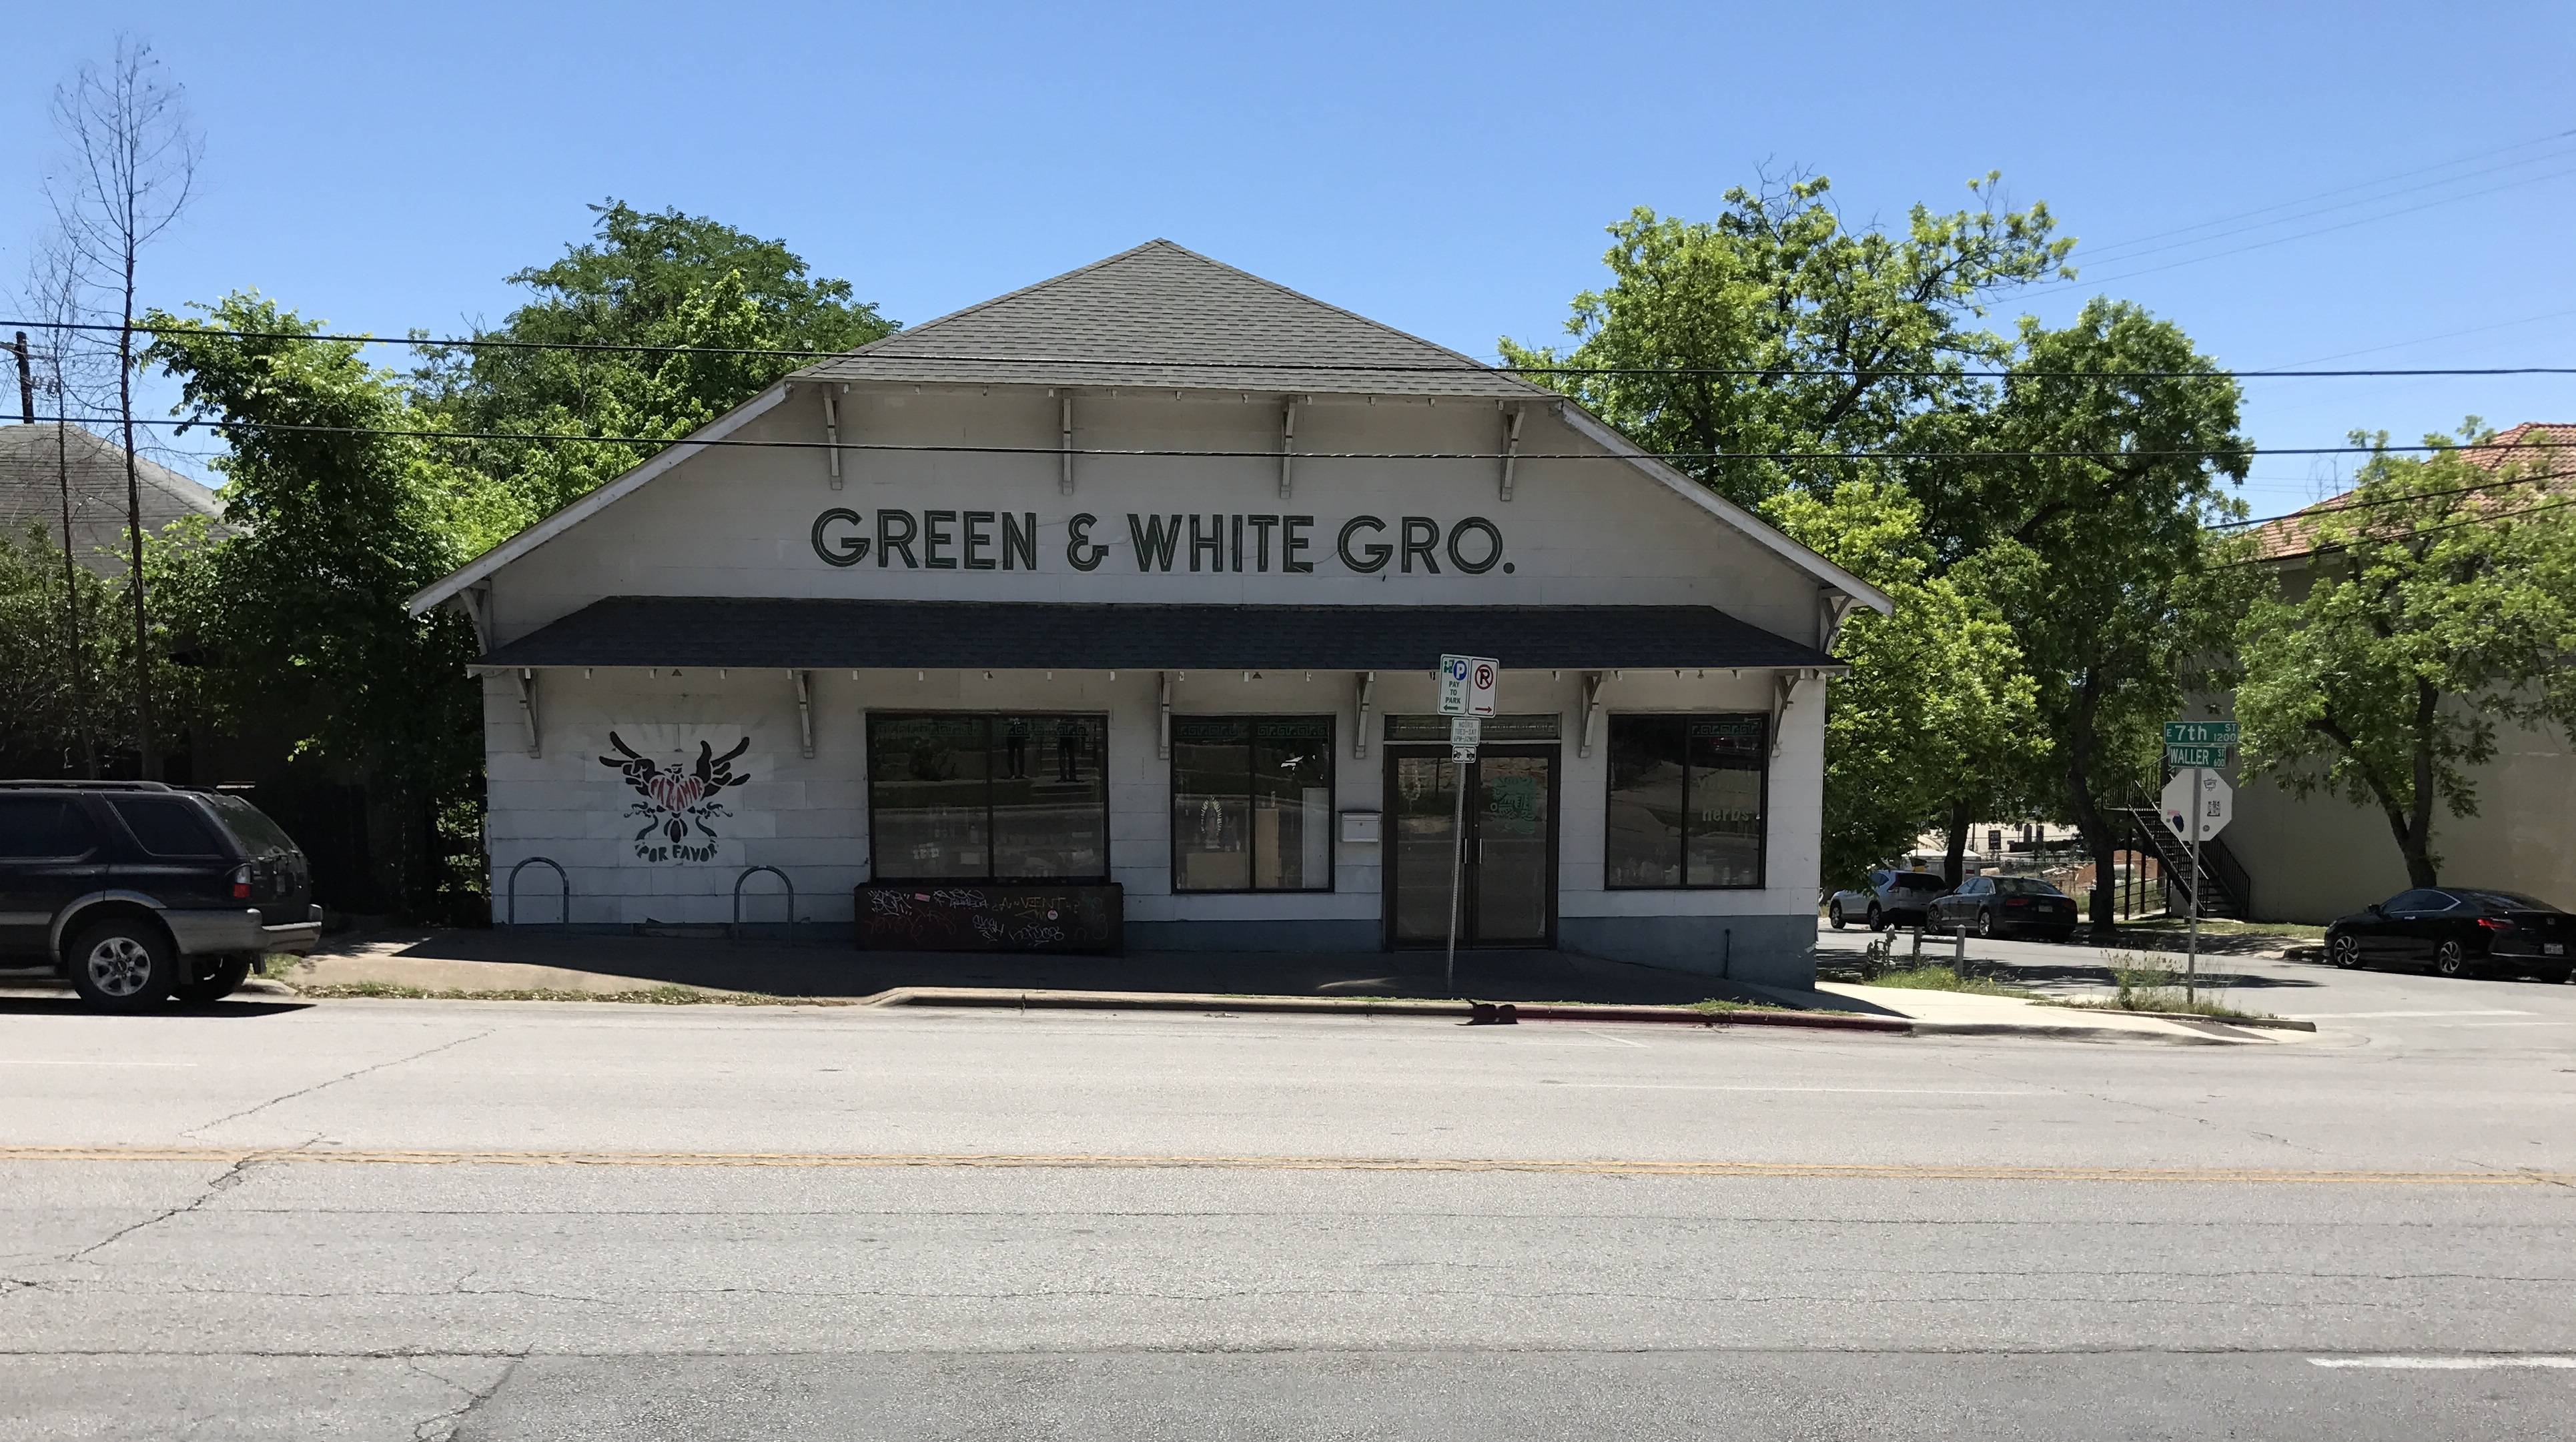
\includegraphics[width=.5\linewidth]{Lindsey_Figure_06}
	\caption{Green and White Grocery northern façade\\
		{\normalfont\scriptsize \copyright\
			\shortauthor
	}}
	\label{fig:Lindsey_Figure_06}
\end{figure}

However, you might start to notice that something is strange about the Green and White Grocery when you see the two Federico Archuleta murals painted in 2014 as Casares recalls (\cref{fig:Lindsey_Figure_07a}, \cref{fig:Lindsey_Figure_07b}). But Archuleta's murals are found on other Mexican-American-owned buildings in Austin, none of them hiding a secret as profound as the Green and White Grocery's. Your first real sign about the true inventory of the Green and White Grocery would be the stylized Aztec eagle on the entrance (\cref{fig:Lindsey_Figure_08}).

%FIGURE 7: Comparison
\begin{figure}[!tb]
	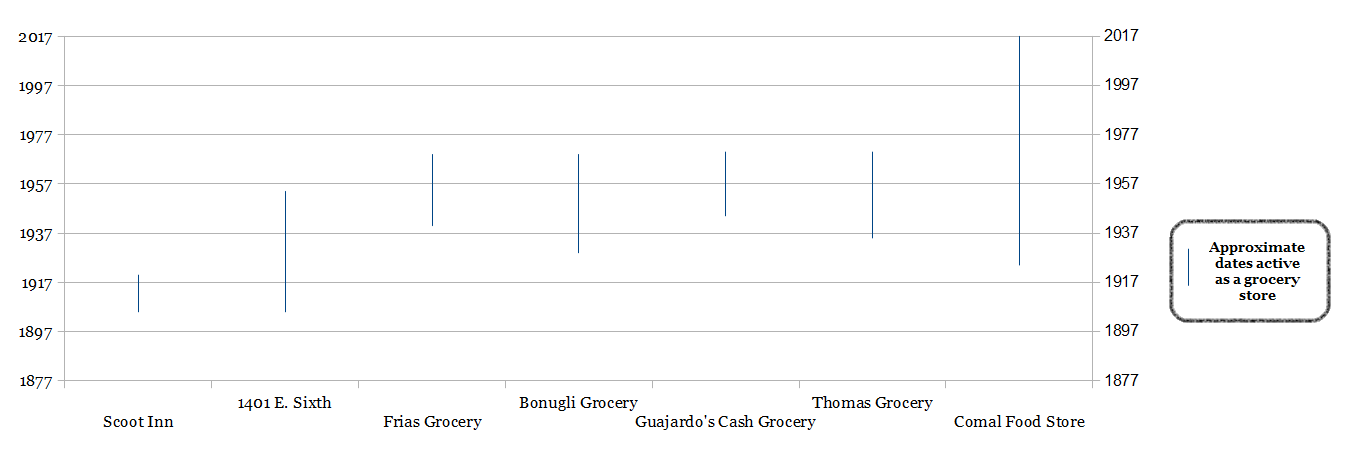
\includegraphics[width=.5\linewidth]{Lindsey_Figure_07}
	\caption{A comparison of relative lengths of time East Austin structures mentioned in the Hardy, Heck, Moore, Inc. (2016) report operated as grocery stores\\
		{\normalfont\scriptsize \copyright\
			\shortauthor
	}}
	\label{fig:Lindsey_Figure_07}
\end{figure}
%missing figure - check with author


%FIGURE 07a: North mural
\begin{figure}[!tb]
	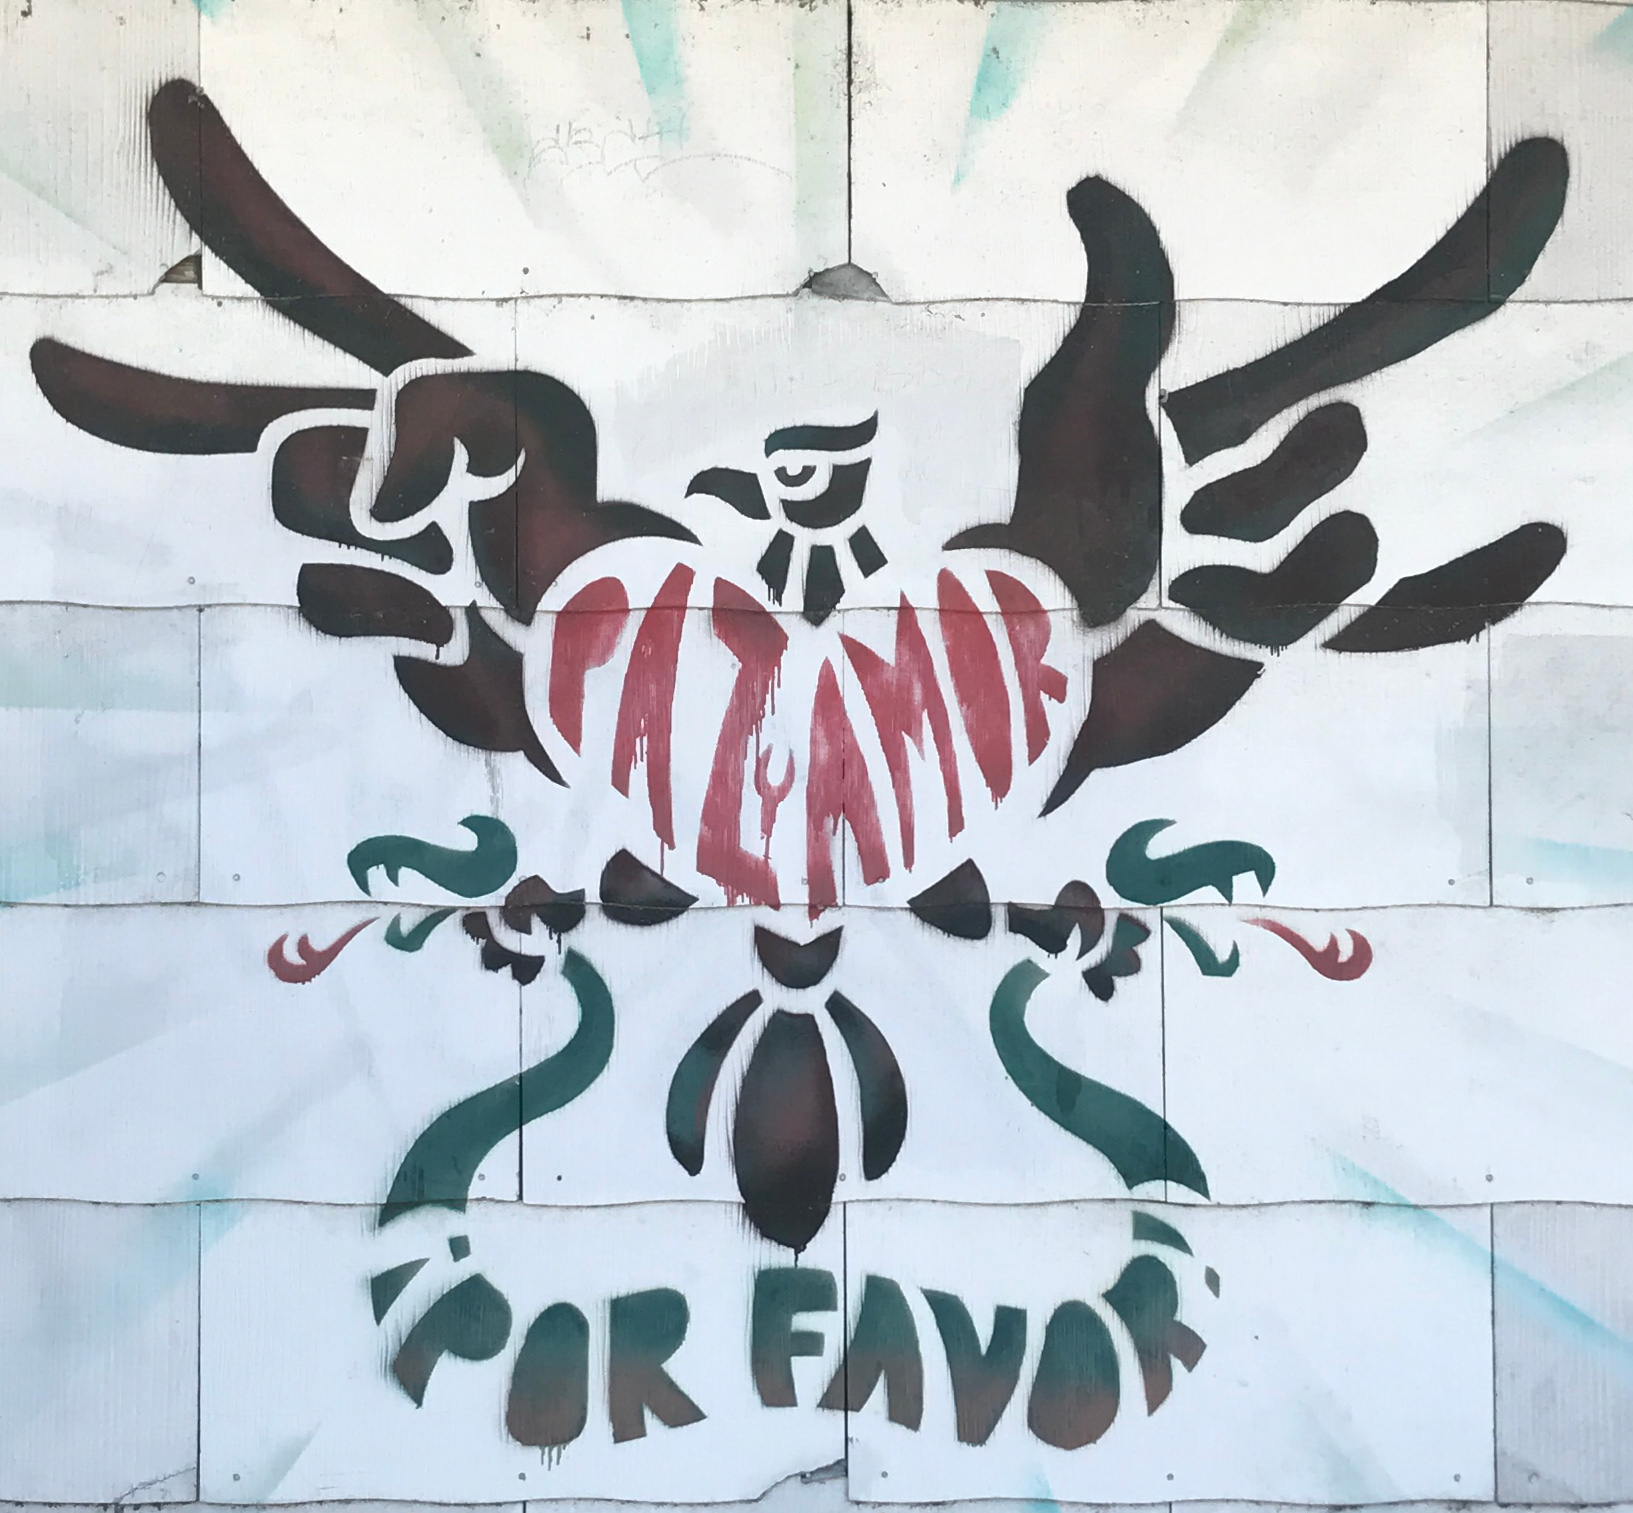
\includegraphics[width=.5\linewidth]{Lindsey_Figure_07a}
	\caption{The north mural by Federico Archuleta\\
		{\normalfont\scriptsize \copyright\
			\shortauthor
	}}
	\label{fig:Lindsey_Figure_07a}
\end{figure}

%FIGURE 07b: West mural
\begin{figure}[!tb]
	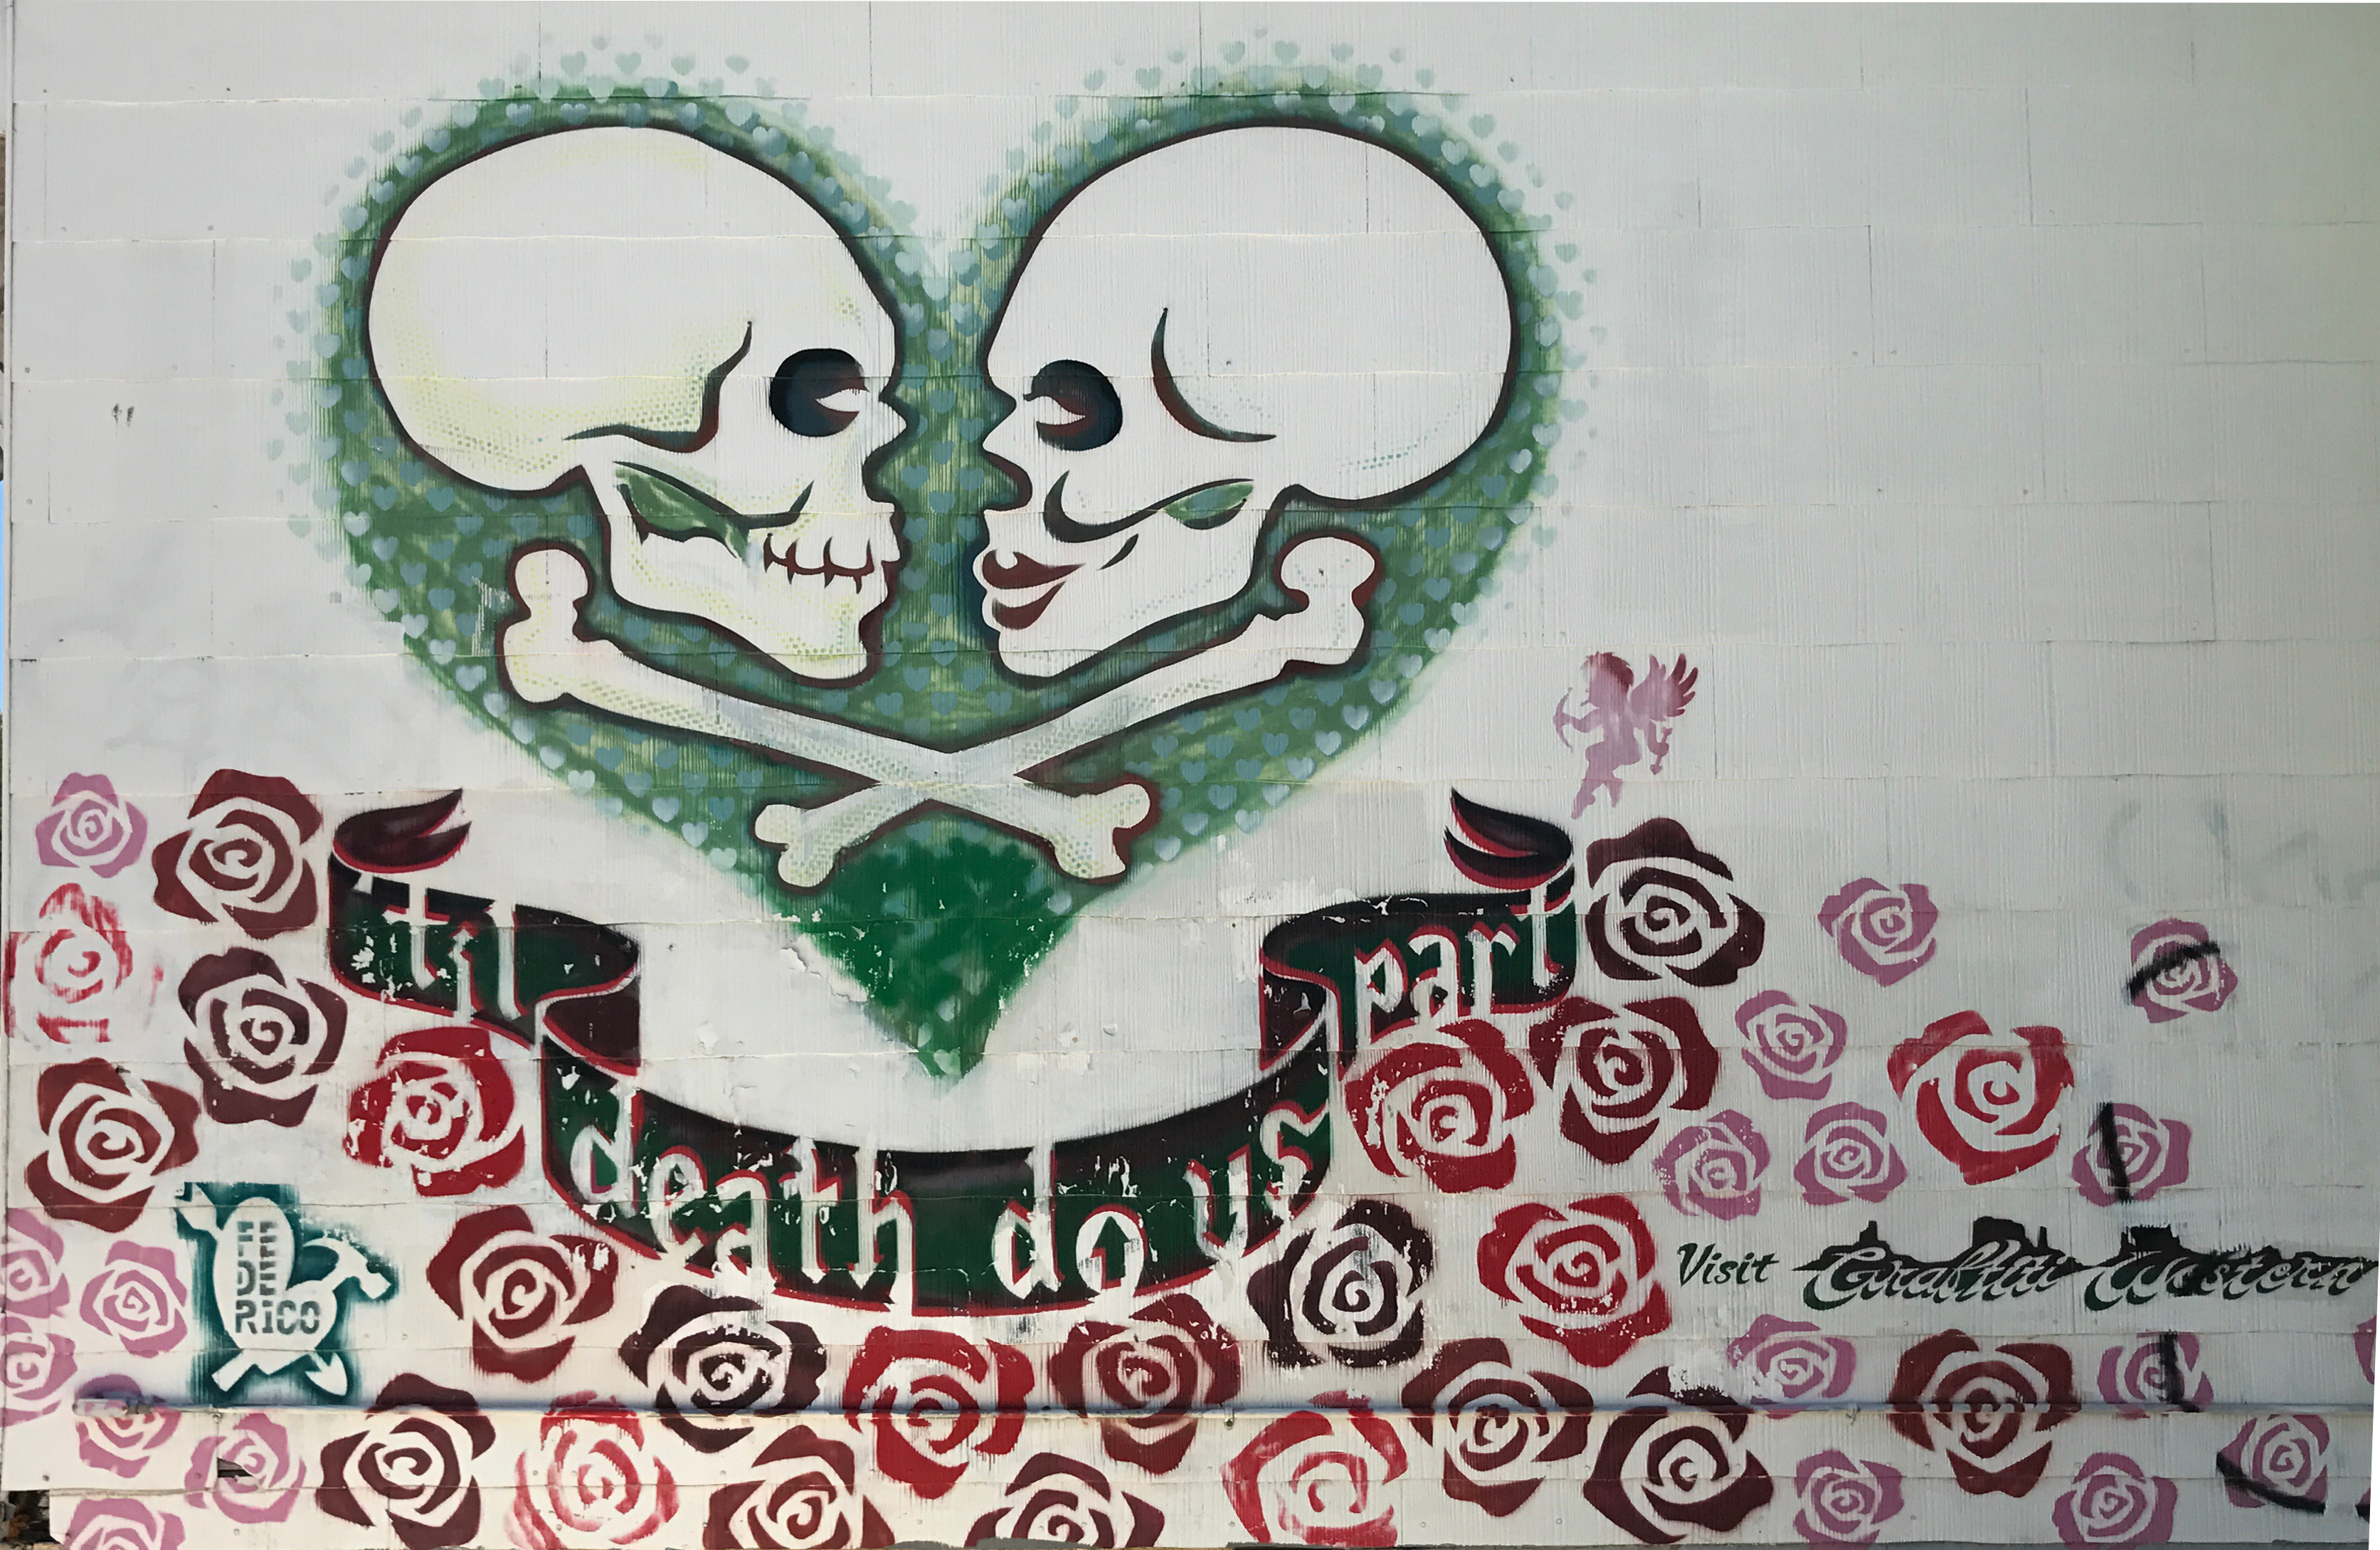
\includegraphics[width=.5\linewidth]{Lindsey_Figure_07b}
	\caption{The west mural by Federico Archuleta\\
		{\normalfont\scriptsize \copyright\
			\shortauthor
	}}
	\label{fig:Lindsey_Figure_07b}
\end{figure}

%FIGURE 08: Aztec eagle
\begin{figure}[!tb]
	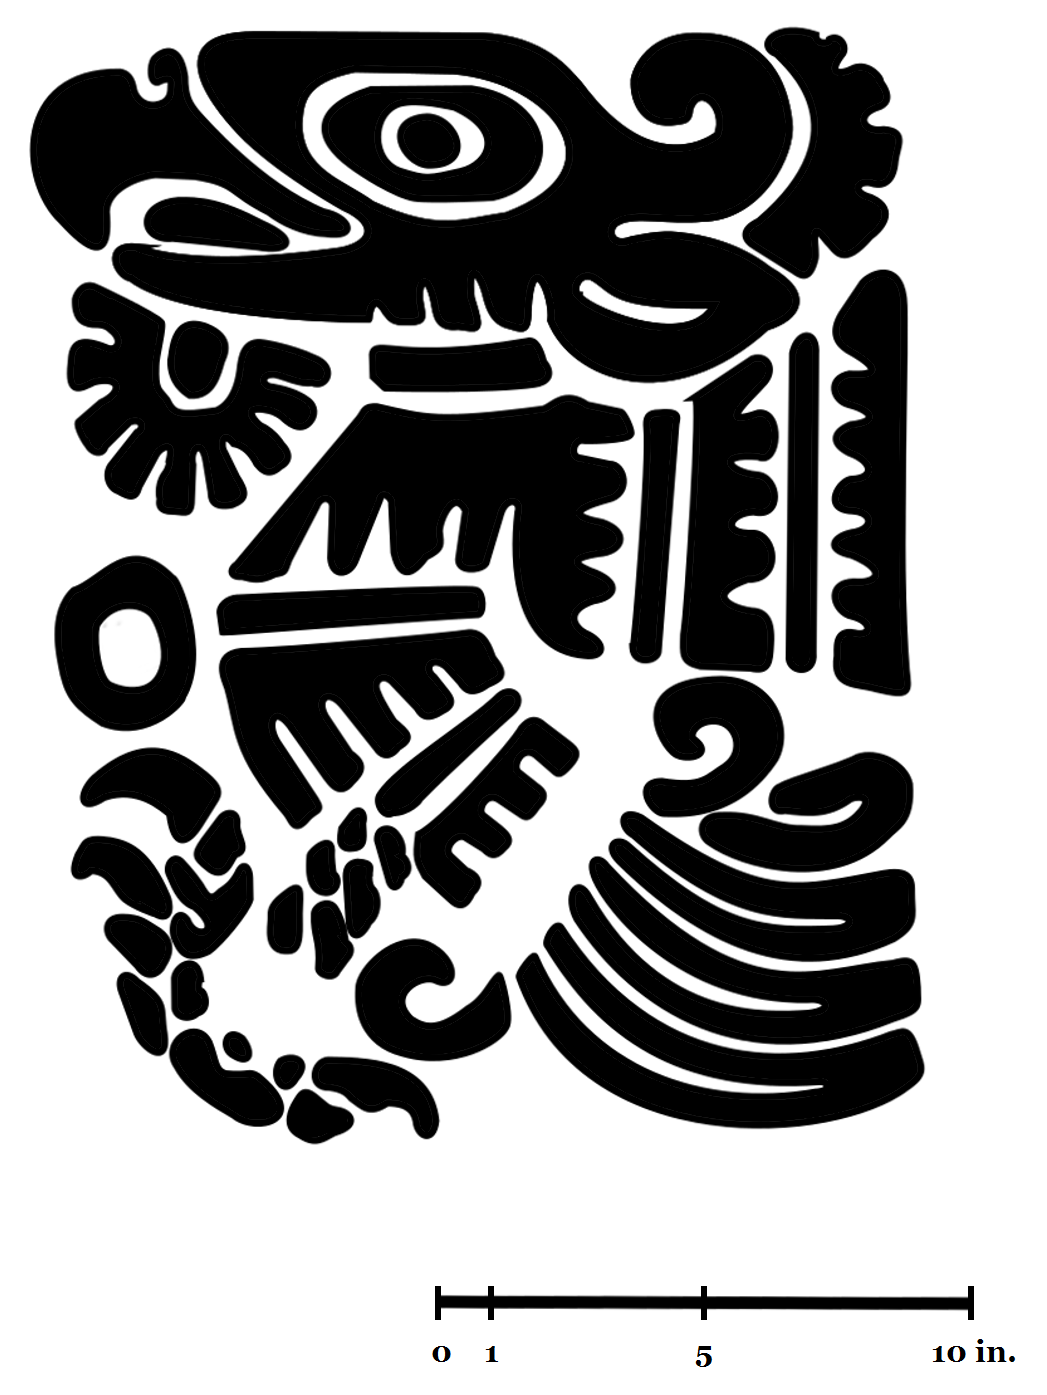
\includegraphics[width=.5\linewidth]{Lindsey_Figure_08}
	\caption{The Aztec-style cuauhtli (eagle) on the door\\
		{\normalfont\scriptsize \copyright\
			\shortauthor rendering
	}}
	\label{fig:Lindsey_Figure_08}
\end{figure}

When you open the door though you will realize the store sells spiritual, not physical, nourishment. Instead of milk, you will find powders, incenses, candles, and statues expressing a variety of personalized religious beliefs. These beliefs are sometimes referred to as syncretic, a term used to describe mixed religious beliefs. However, practitioners often do not see their beliefs as a mixture of systems but a singular, coherent, and personalized system (\cites{romberg1998}{romberg2005}). Instead, ‘Spiritist’ may be more appropriate, as it implies belief in a spirit world but does not confine the system to beliefs from specific regions (\cite{romberg2005}). Objects for sale in the store include saint candles of Mexican Catholic tradition, representations of Mesoamerican ceremonial death masks, and even iconography from other world religions.

%FIGURE 09: Overview
\begin{figure}[!tb]
	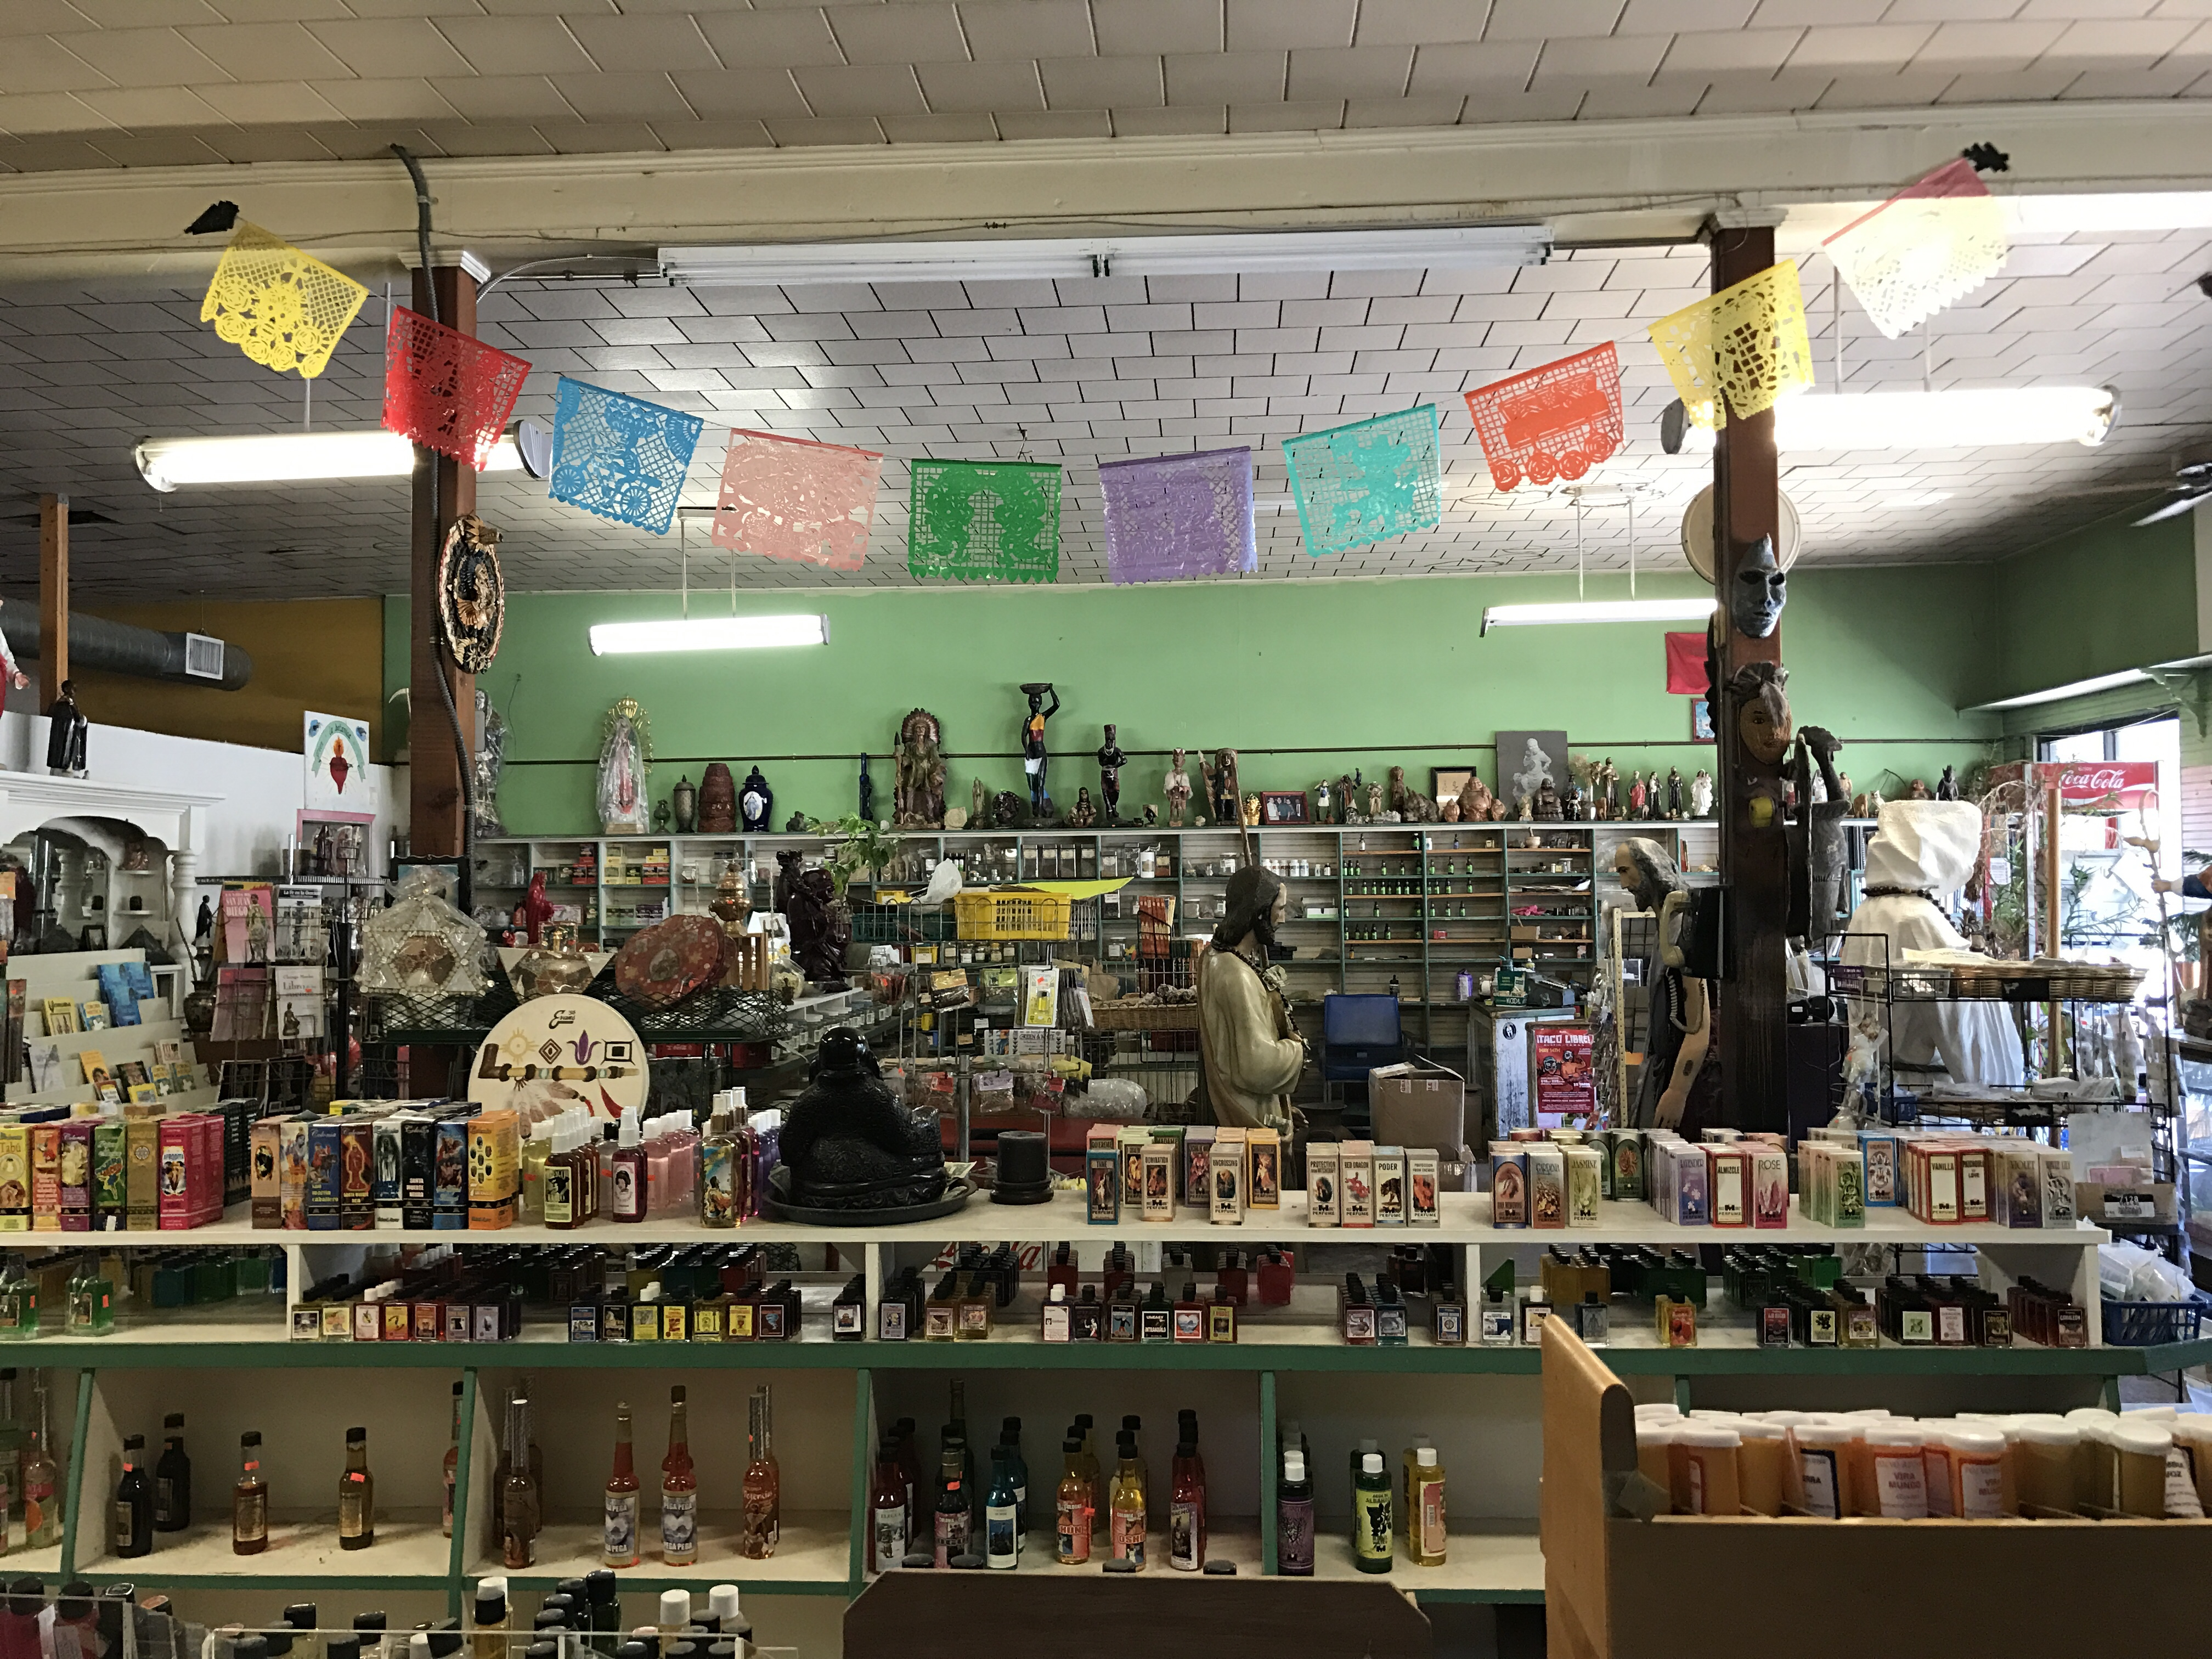
\includegraphics[width=.5\linewidth]{Lindsey_Figure_09}
	\caption{Overview of store space\\
		{\normalfont\scriptsize \copyright\
			\shortauthor
	}}
	\label{fig:Lindsey_Figure_09}
\end{figure}

The majority of objects, from candles and statues of Christian saints to incense from the copal tree, represent local or indigenous Mexican, Mexican-American, and Chicano spiritual beliefs. Many of them are representative of the history woven by Chicanx philosophers, as they mix pre-Hispanic Mesoamerican values with the Spanish Catholic imagery. In Chicano philosophy, the use of pre-contact Mesoamerican imagery is a way of maintaining a distinct identity within broader U.S. culture (see, for example, \cite{anzaldua}).

Location was important in pre-contact Mesoamerica. The ancient Maya connected with their ancestors at specific sacred temples, Teotihuacanos buried important ancestors under the floor often with masks similar to the ones on display at the Green and White Grocery, and the ancient Mixtecos cremated their ancestors to keep them close (\cites[184]{ashmore}{linne}[7]{joyce}). All these practices share the core belief that places are sacred. And it is through families that places are imbued with energy over generations. What was once a grocery store now is firmly an herbal shop, a botánica. Yet, like the temples of the pre-contact people of Mexico, it has neither resisted change nor lost the basic elements which make it important to its users.

%FIGURE 10: Shelving
\begin{figure}[!tb]
	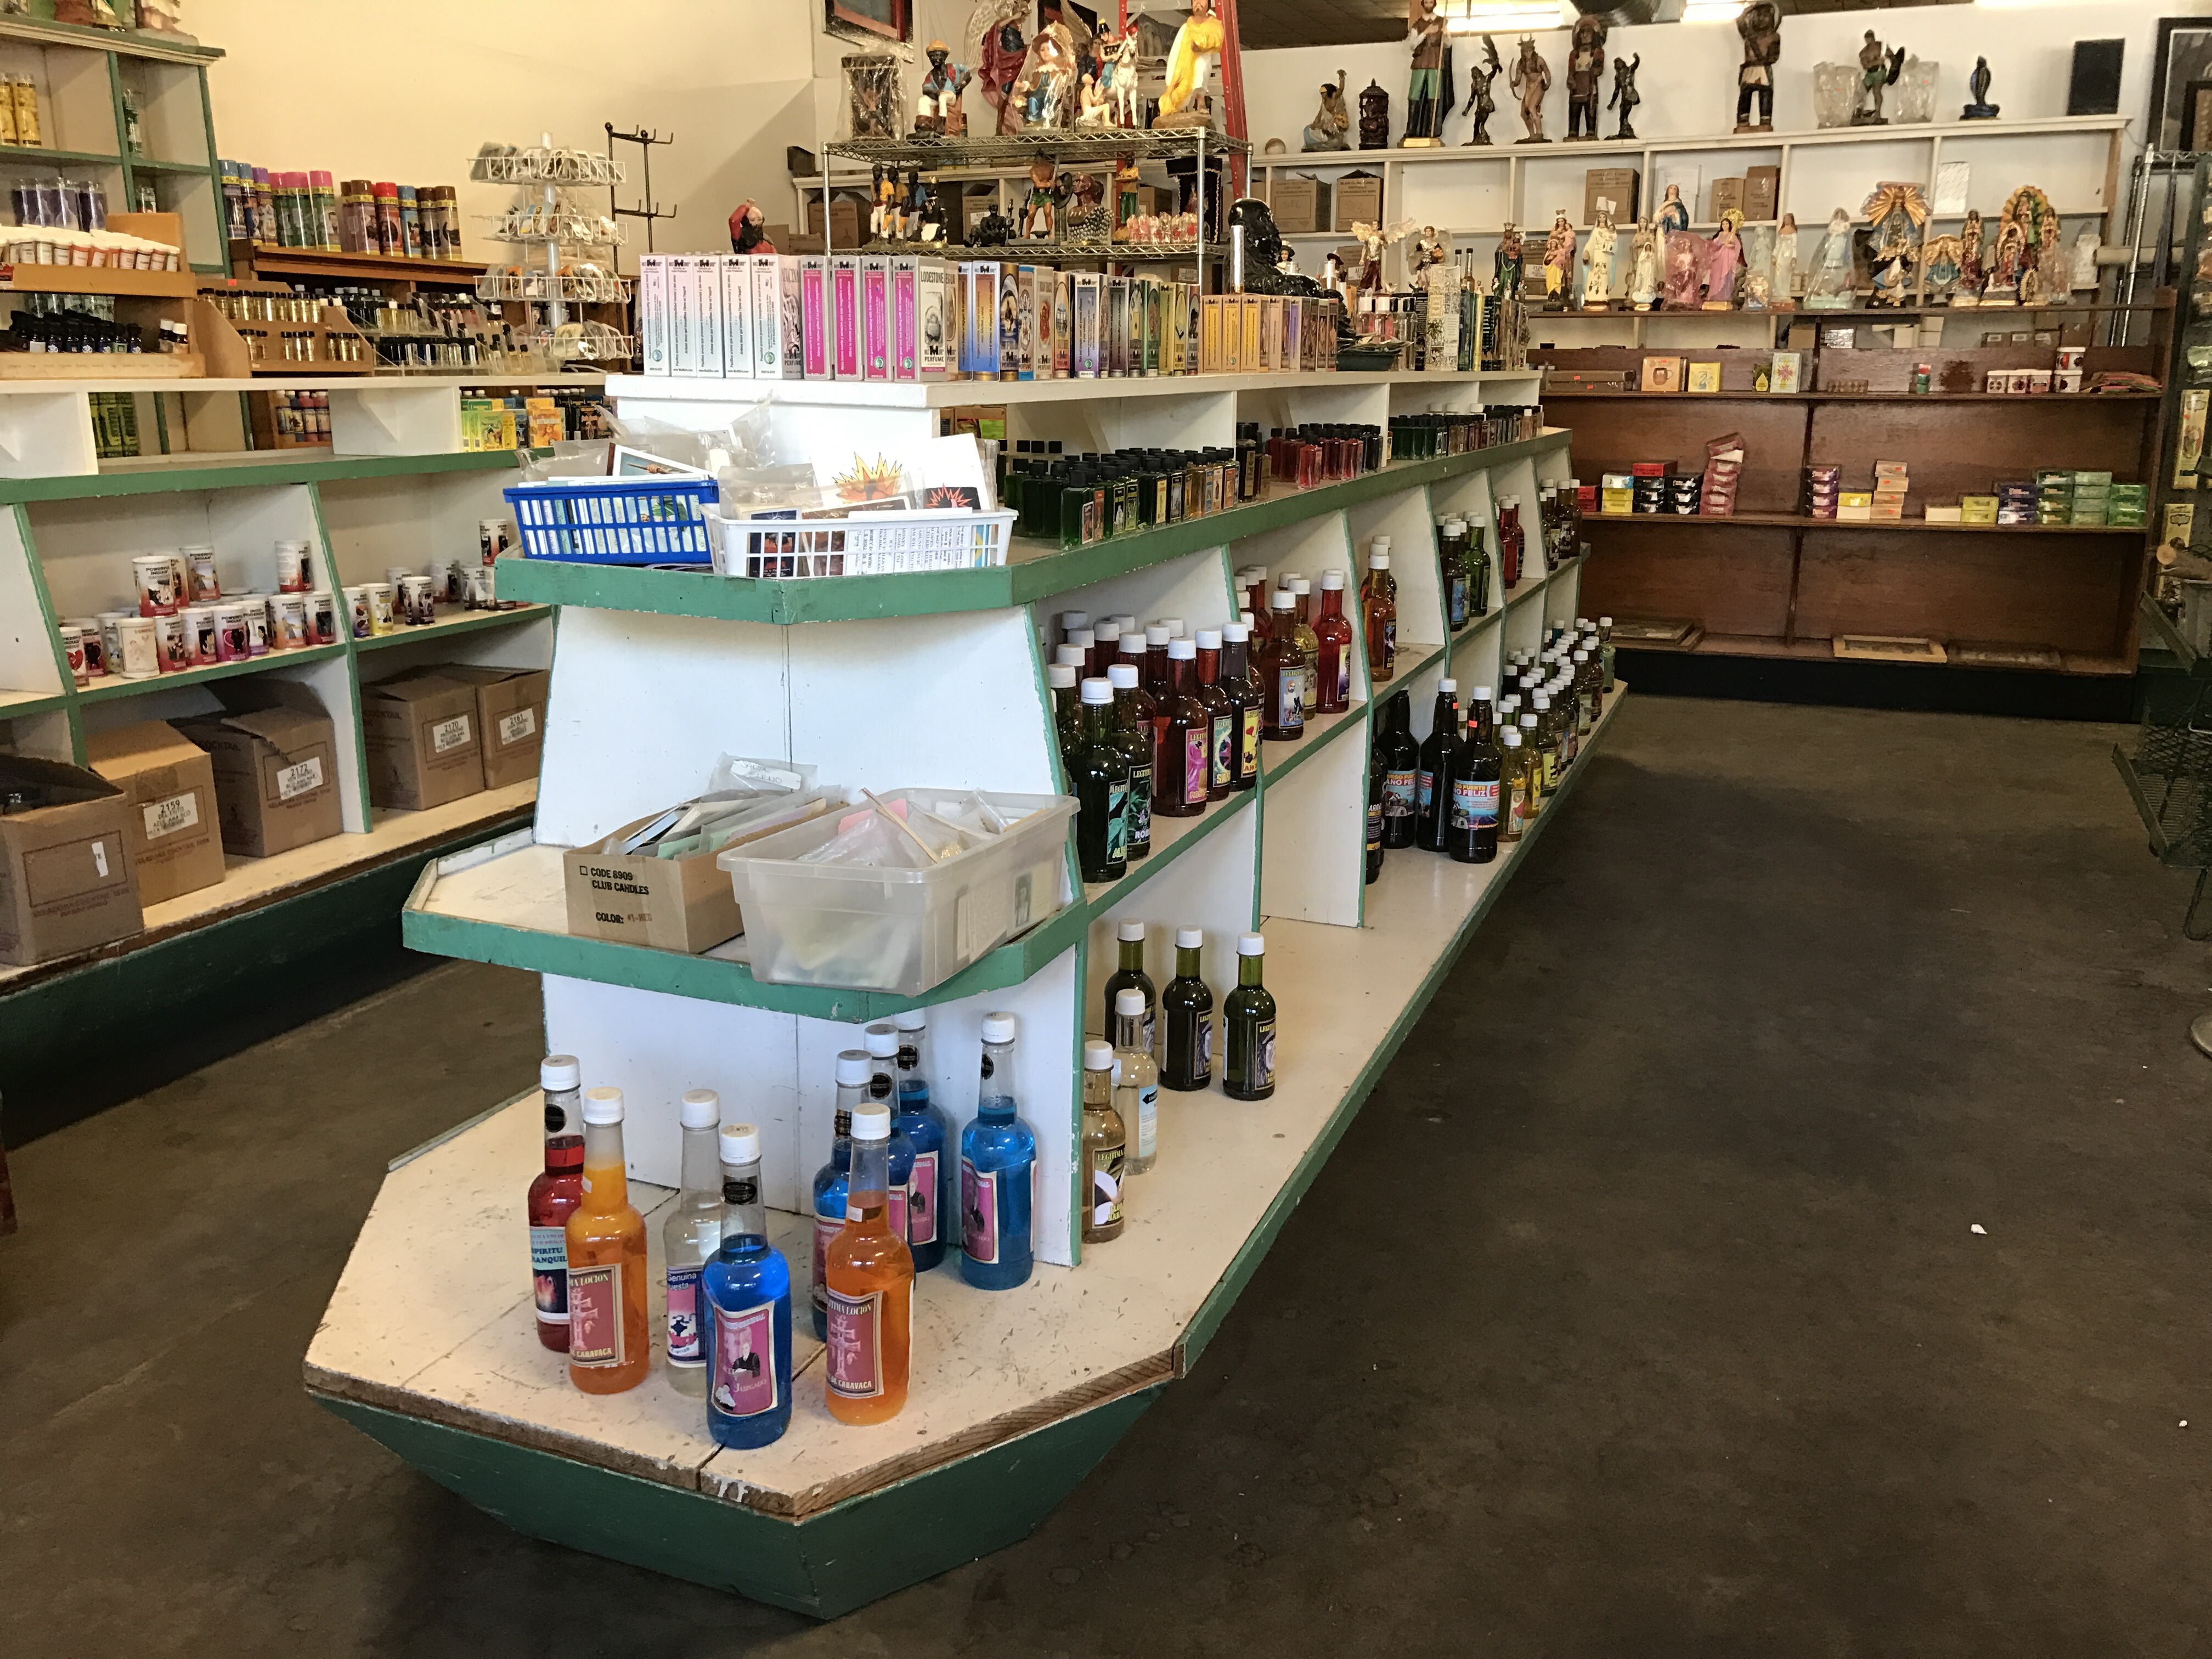
\includegraphics[width=.5\linewidth]{Lindsey_Figure_10}
	\caption{Original shelving\\
		{\normalfont\scriptsize \copyright\
			\shortauthor
	}}
	\label{fig:Lindsey_Figure_10}
\end{figure}

This is more than poetic divergence. The two biggest alterations to the building itself, an extension and a roof remodeling, were both in the building's early history. What we see today is what John has known for most of his life. This includes the shelving, which provides a circuit for customers leading down all the aisles and to the cash register.

%FIGURE 11: Foot traffic
\begin{figure}[!tb]
	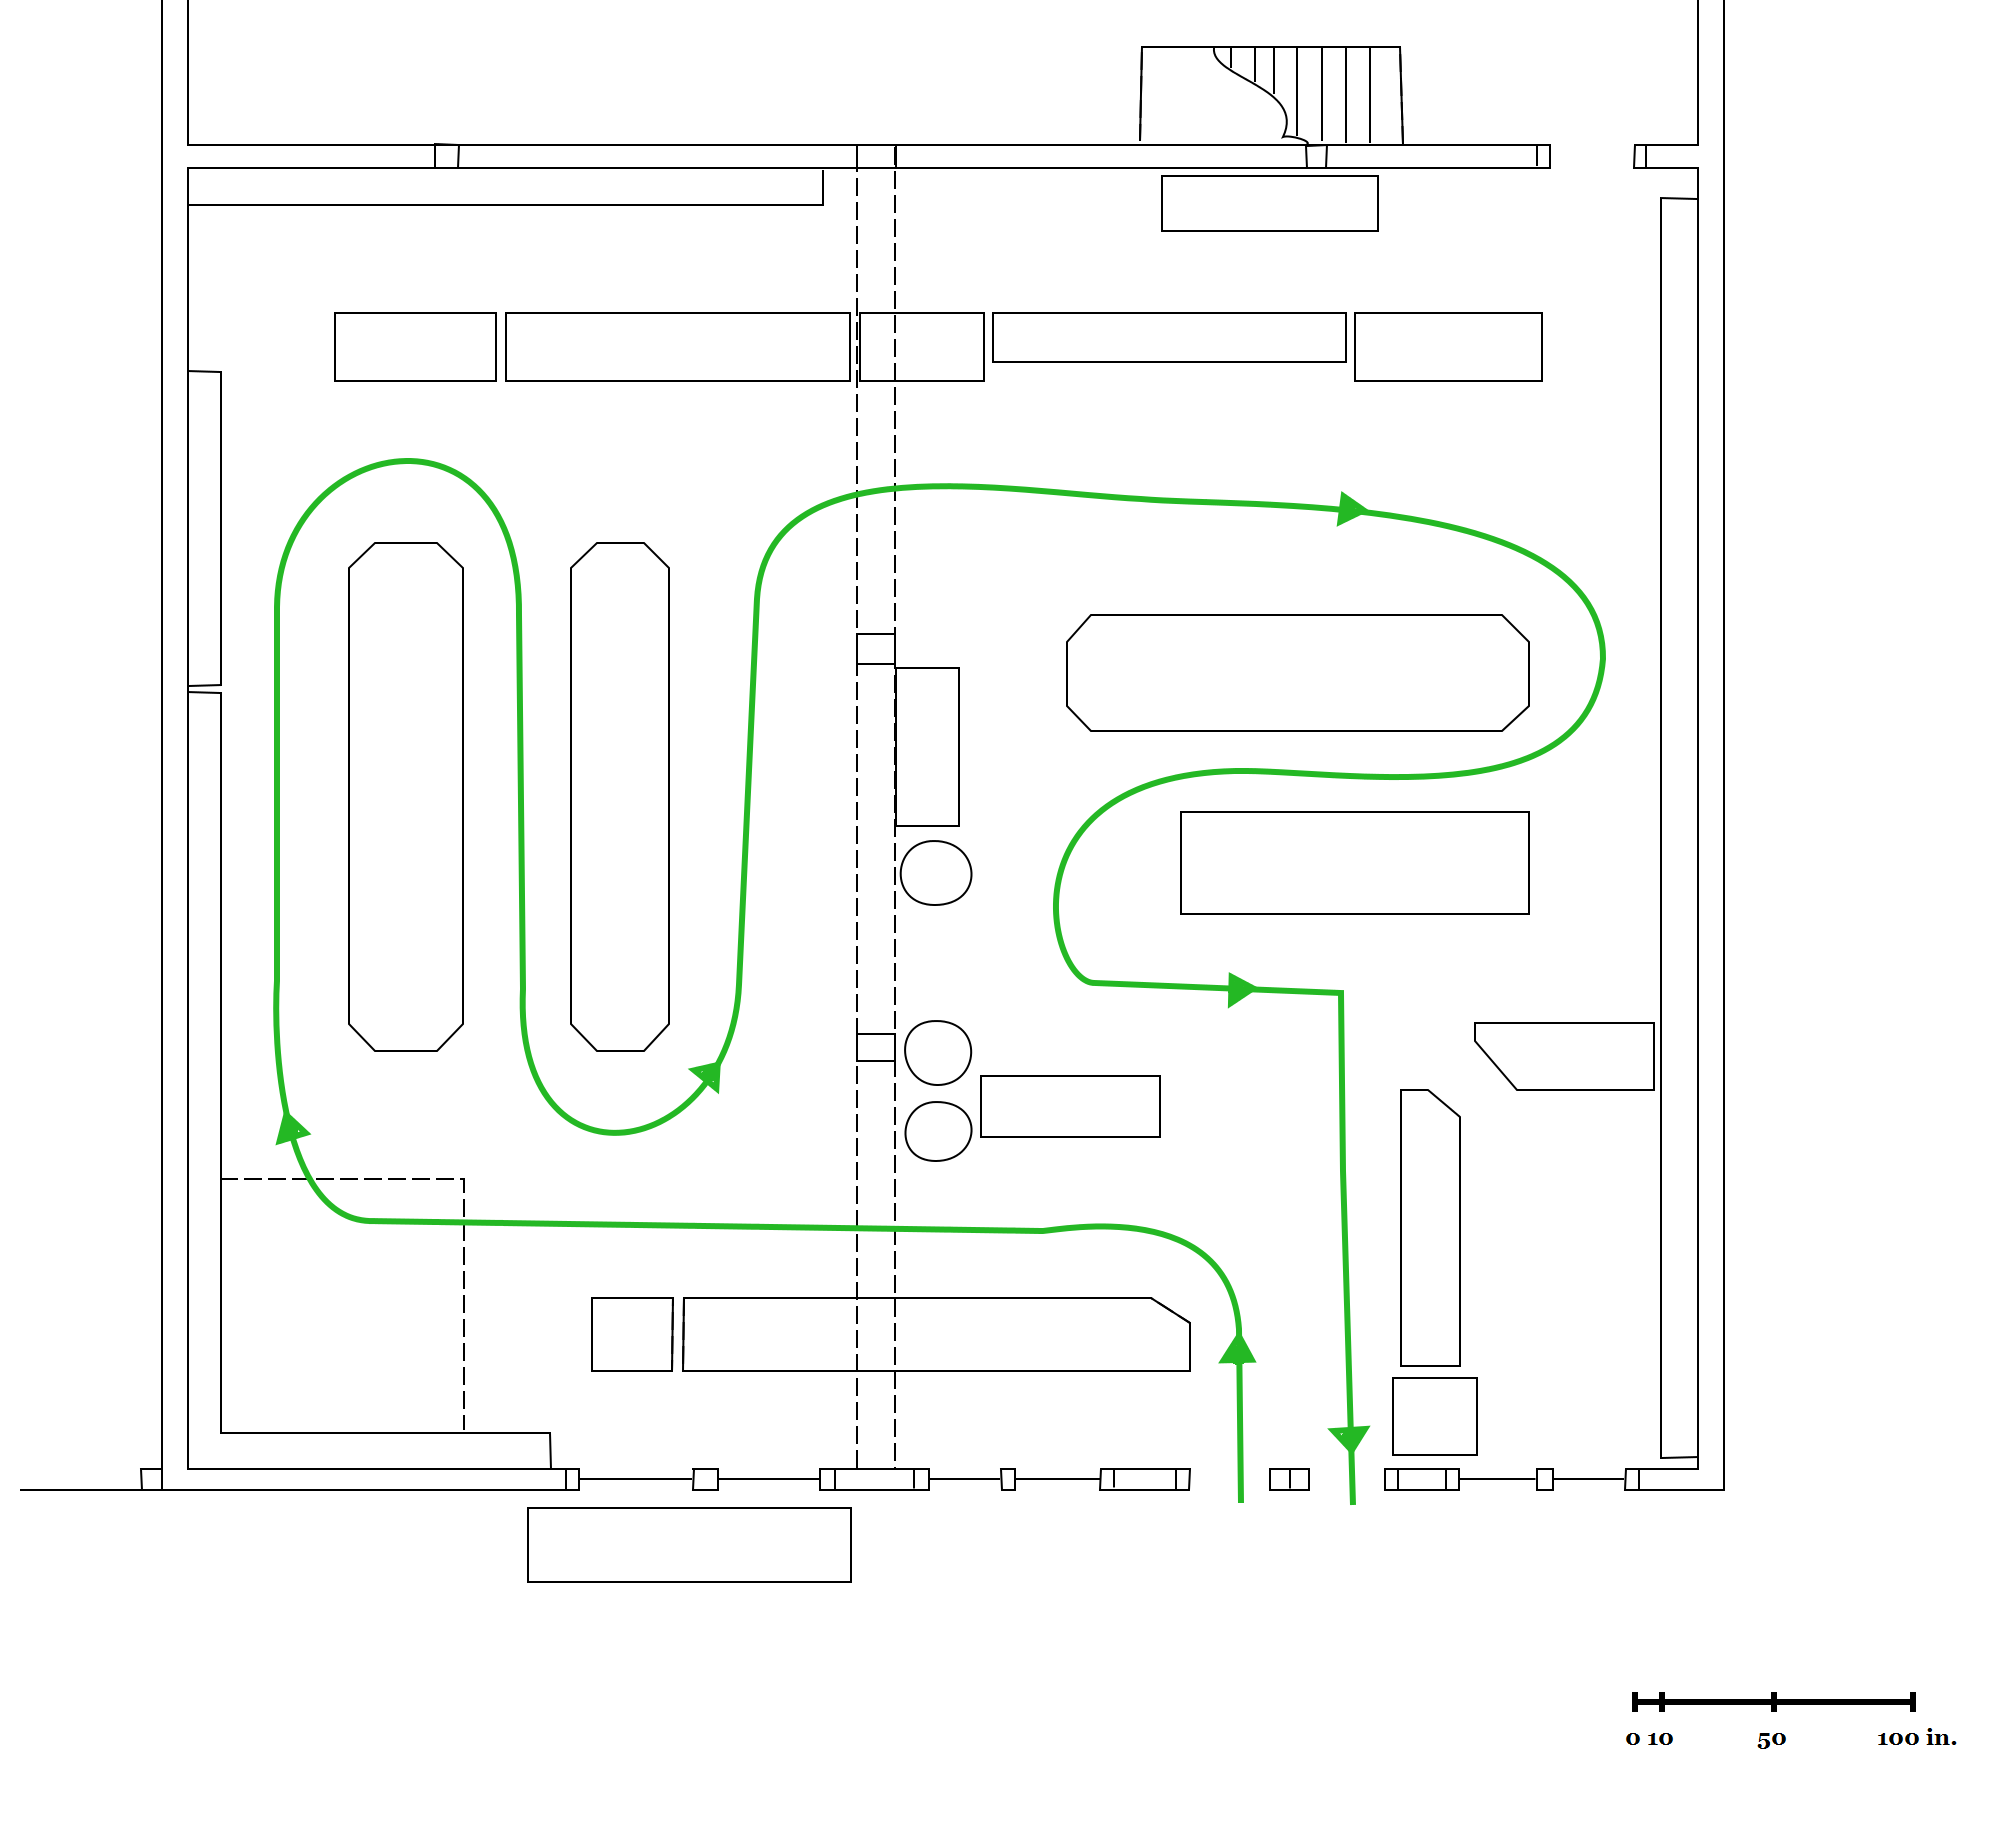
\includegraphics[width=.5\linewidth]{Lindsey_Figure_11}
	\caption{One potential foot traffic map allowing customers to interact with almost all shelving without disruption\\
		{\normalfont\scriptsize \copyright\
			\shortauthor, illustration
	}}
	\label{fig:Lindsey_Figure_11}
\end{figure}

Most buildings control access to some extent or another (\cites{campion}[52]{glassie}), and in this way the Green and White Grocery has resisted change. A customer visiting the Green and White Grocery in 1958 would have had the same relative access points: a tree blocked access to the east side as the gate does today; the Green and White Grocery sits on a corner lot, exposing two sides of the building to sidewalk; and only one of these sides permits access: the north side. Though the main doorway was replaced in the 1980s, it remains at the same location, and though the ice box was removed, this was never an access point to the interior.

%FIGURE 12: Ice box
\begin{figure}[!tb]
	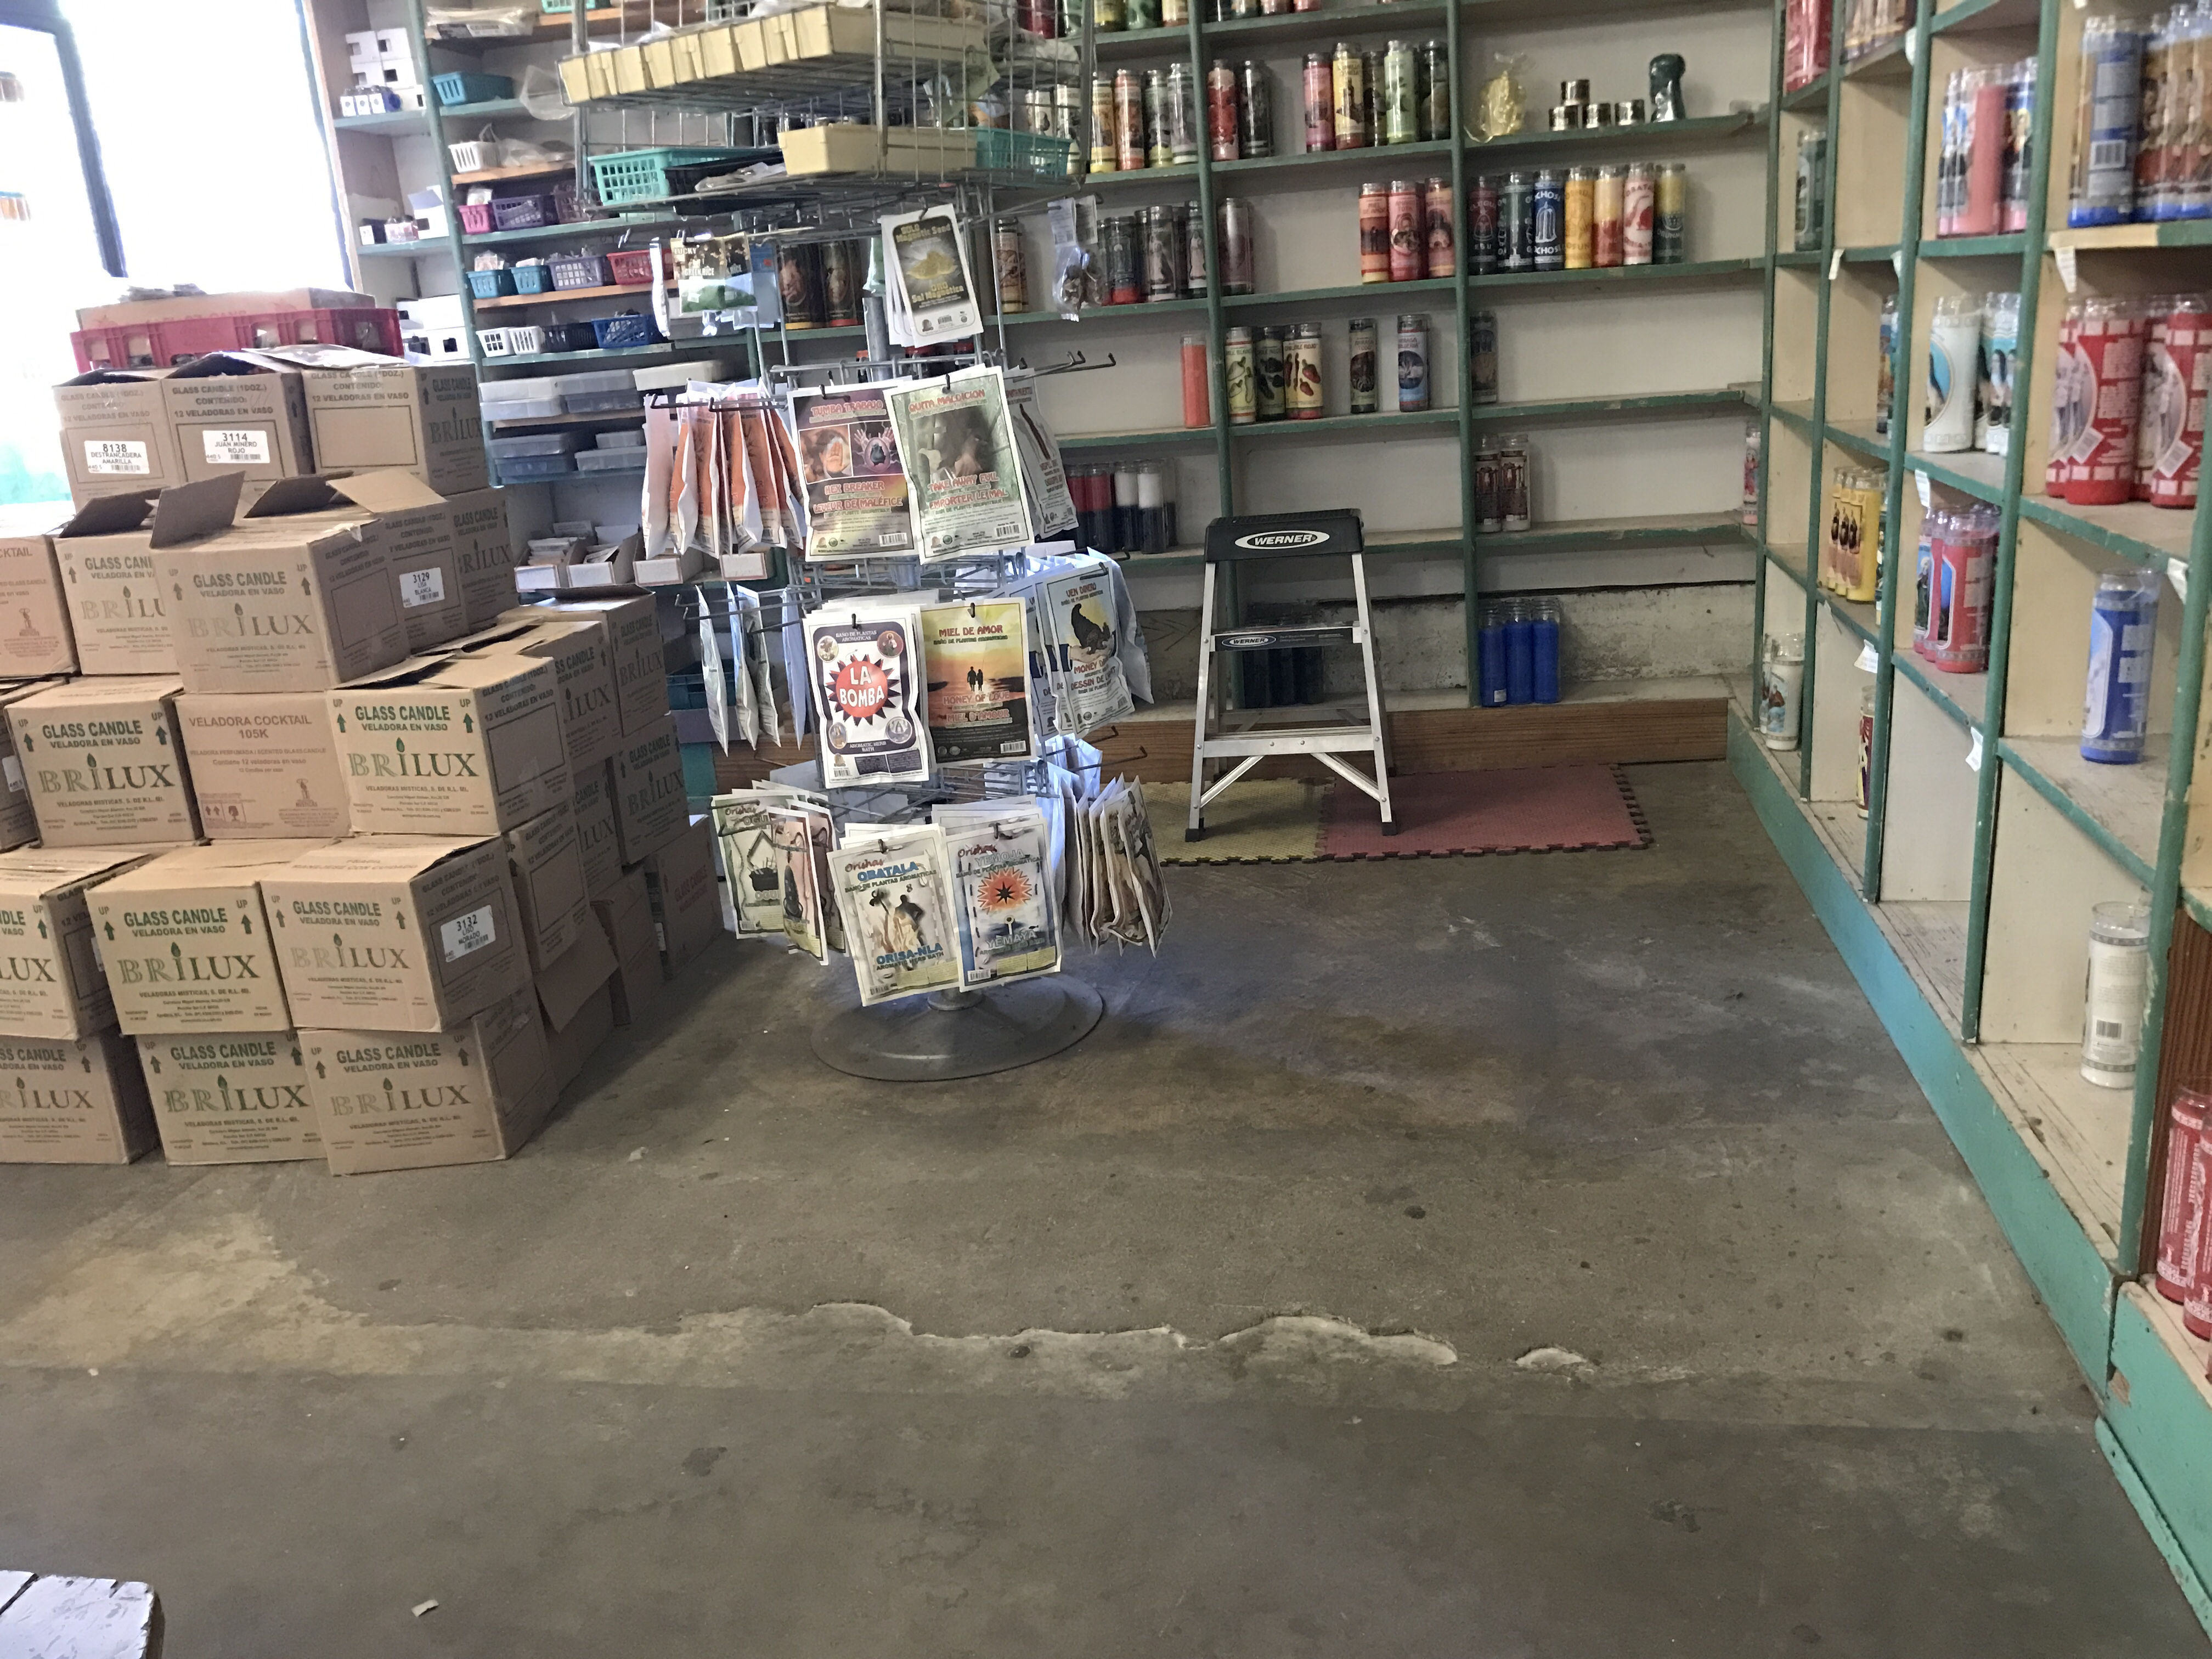
\includegraphics[width=.5\linewidth]{Lindsey_Figure_12}
	\caption{Disruption in concrete fabric indicating removed ice box\\
		{\normalfont\scriptsize \copyright\
			\shortauthor, illustration
	}}
	\label{fig:Lindsey_Figure_12}
\end{figure}

Early customers also could have bought the candles, incenses, and other religious paraphernalia that make up the entirety of the Green and White Grocery's inventory today. Casares recalls that Noberto and Susie Lopez imported candles and incenses from the same distributor who provided them with foodstuffs. Over the years Cazares has moved away from food, but the legacy of those days is still obvious right down to two old Coca-Cola coolers.

This is not to deny that important changes have happened at the store, but they appear to be measured, deliberate changes. In 2003, Cazares told the East Austin Project, \blockcquote{becker}{I'm still learning, and all my practices are going to keep me learning, because you never know everything, and you never refine anything. It's a constant refinement}. Even since then, the storefront has changed: Archuleta painted his murals and a newspaper vending machine in the East Austin Project’s two videos has been replaced with a flower planter. But most changes are minor, resulting from basic upkeep. The GREEN \& WHITE GRO. logo, for example, though maintained with new paint, is the same lettering style as in the 1958 photograph (\cref{fig:Lindsey_Figure_04}). Besides the removal of the ice box, the most drastic change visible in the 1958 photograph is a change to the slope of the roof. The Green and White Grocery is recognizable for its double set of eaves: the lower eaves shade entry to the store, while the higher eaves serve as the natural outcropping of the roof.

%FIGURE 13: Eaves
\begin{figure}[!tb]
	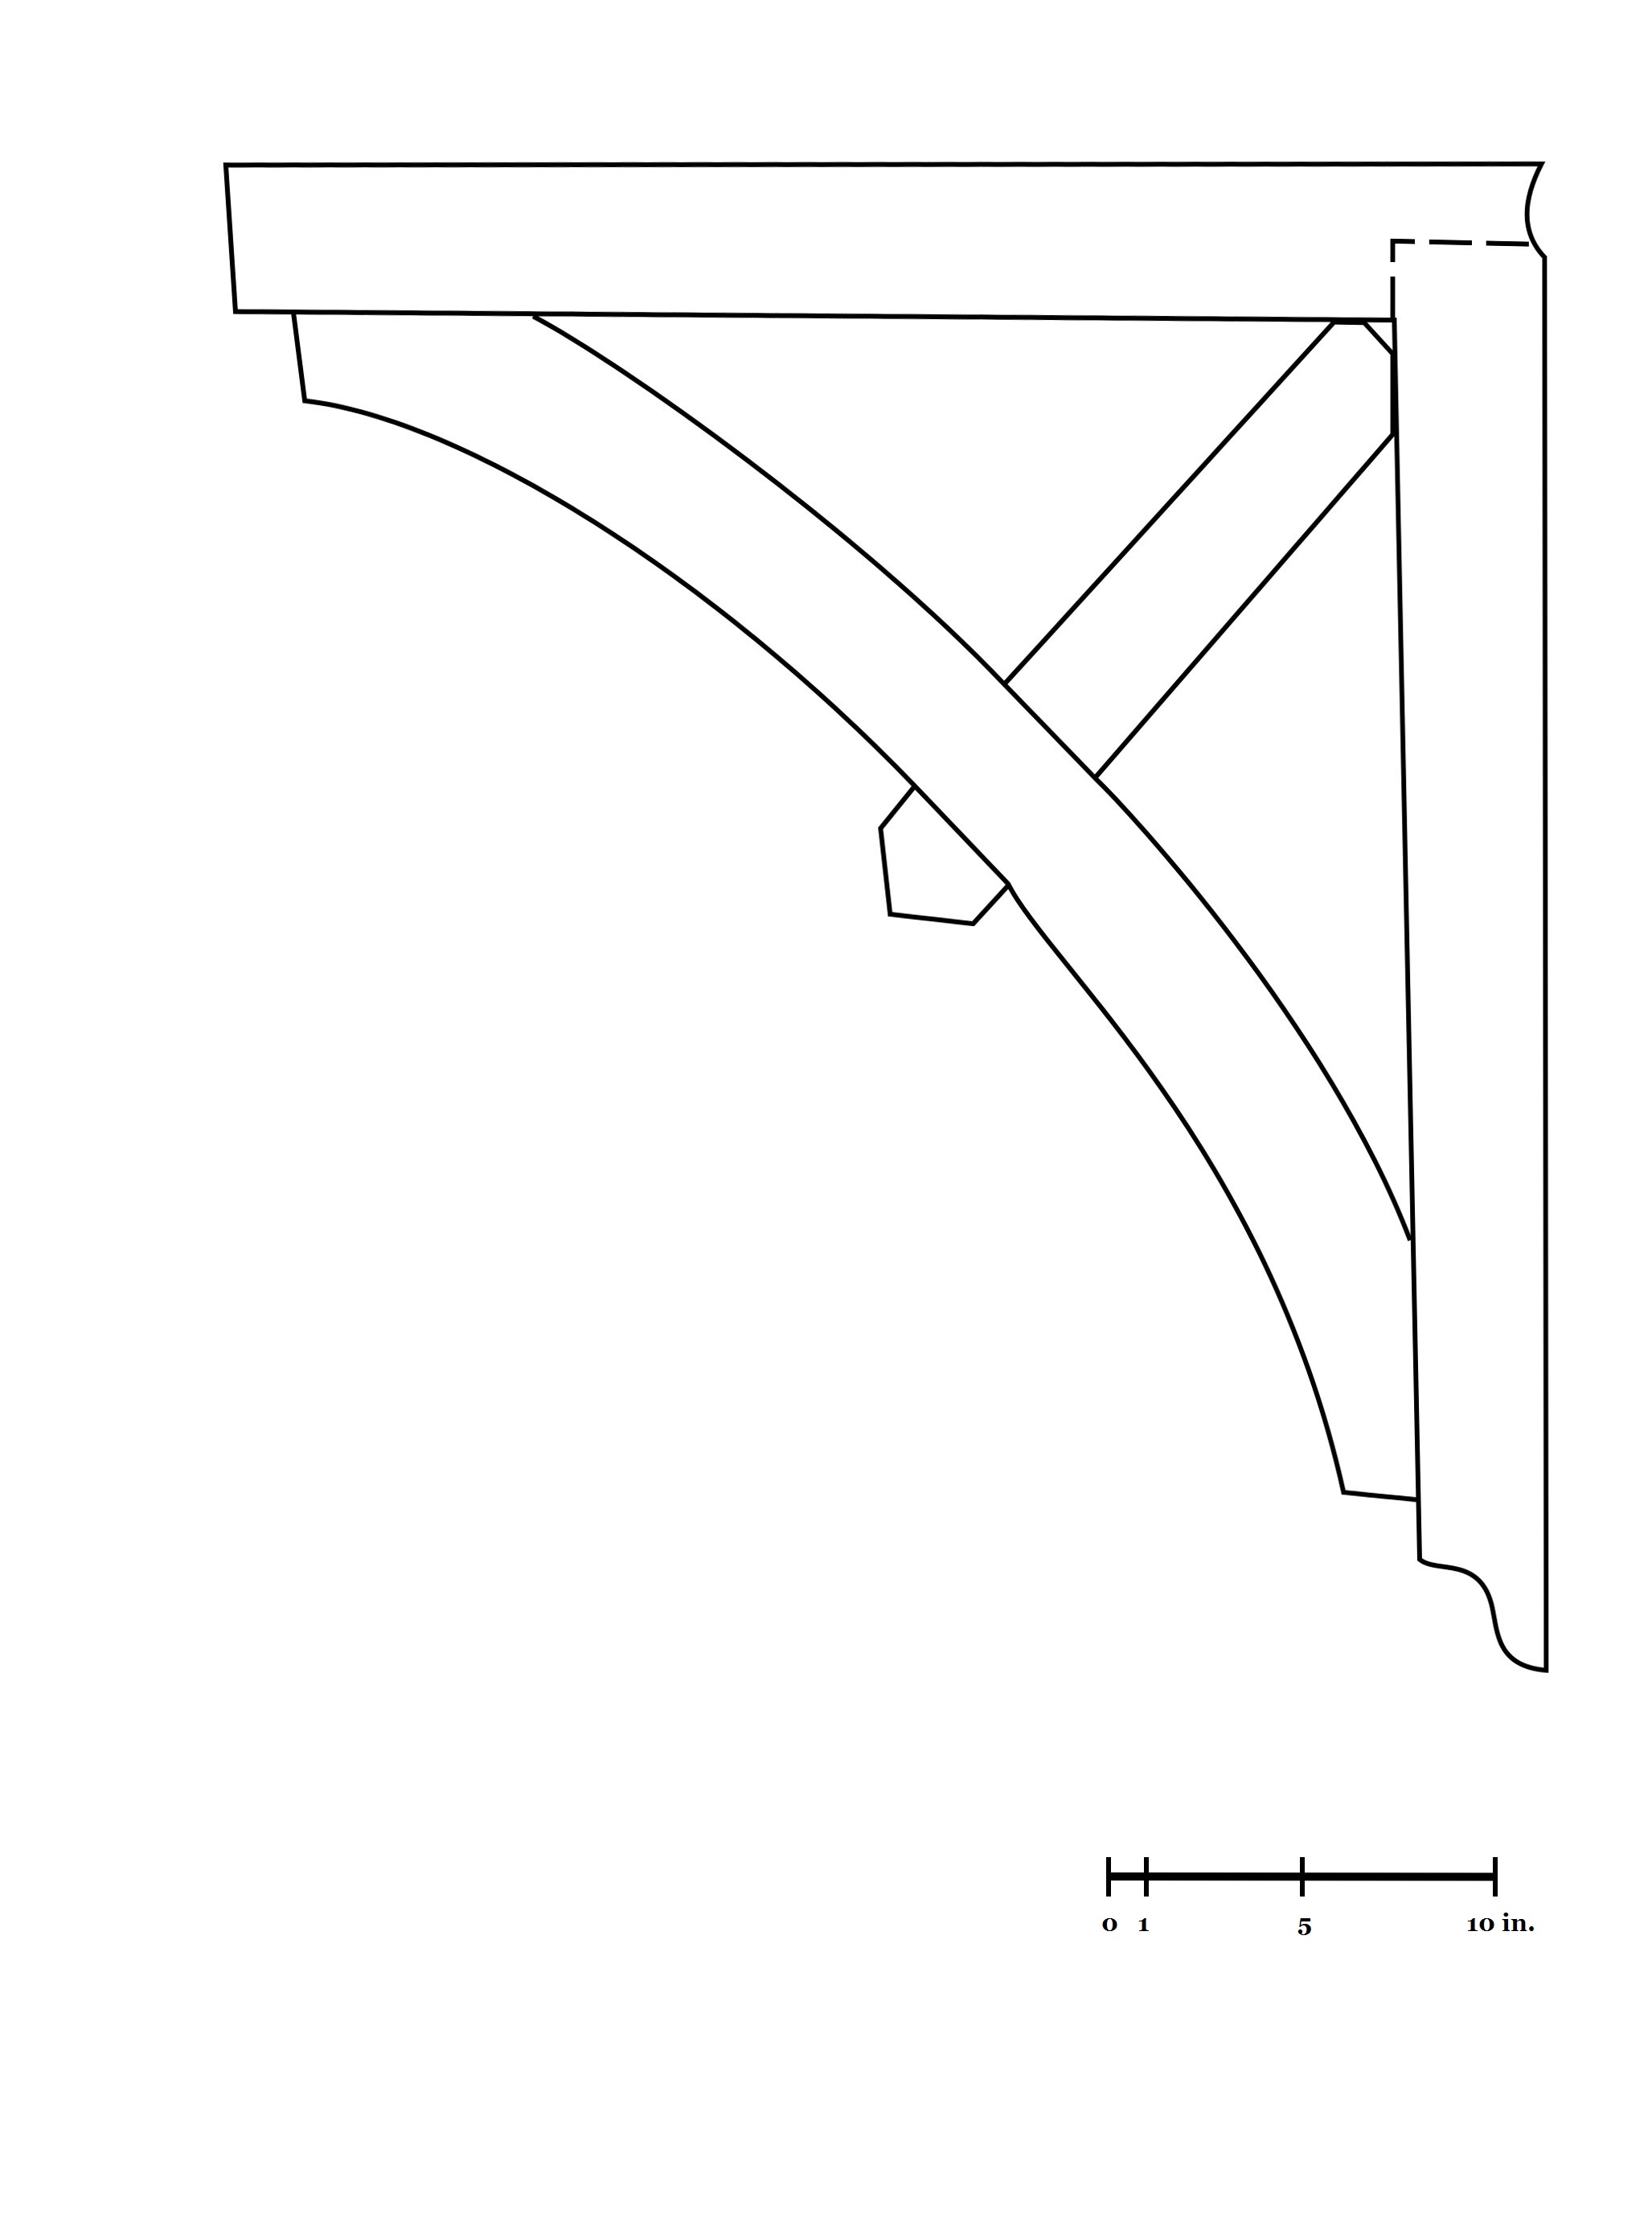
\includegraphics[width=.5\linewidth]{Lindsey_Figure_13}
	\caption{Eaves bracket, lower eaves. The dotted line represents presumed cut of wood based on other brackets; paint was too thick to measure confidently\\
		{\normalfont\scriptsize \copyright\
			\shortauthor, illustration
	}}
	\label{fig:Lindsey_Figure_13}
\end{figure}

The photograph (\cref{fig:Lindsey_Figure_04}) shows this to be a legacy of the building's original form. However, the original higher eaves were restricted to the center of the facade and about a fourth of the length of the wall to either side. The sloped roof was extended, eliminating the “Old West” flat facade of the original building. This probably occurred shortly after the photograph was taken because Cazares did not remember it, noting that in his time he has only maintained but not altered the roof.  As for the rear addition reported by \textcite[75-76]{hardy}, little internal evidence exists for it today and Cazares was unaware of it. Though the outside west wall shows a discontinuity in material use for the foundation (toward the back of the building, it turns to rubble), this does not equate to an internal change in wall or floor pattern. (However, the inside floor at the discontinuity is wooden.) The floor in the southernmost rooms of the structure-which is concrete-appears similar to the floor in the northernmost portions, again making statements about an extension difficult.

%FIGURE 14: Fabric
\begin{figure}[!tb]
	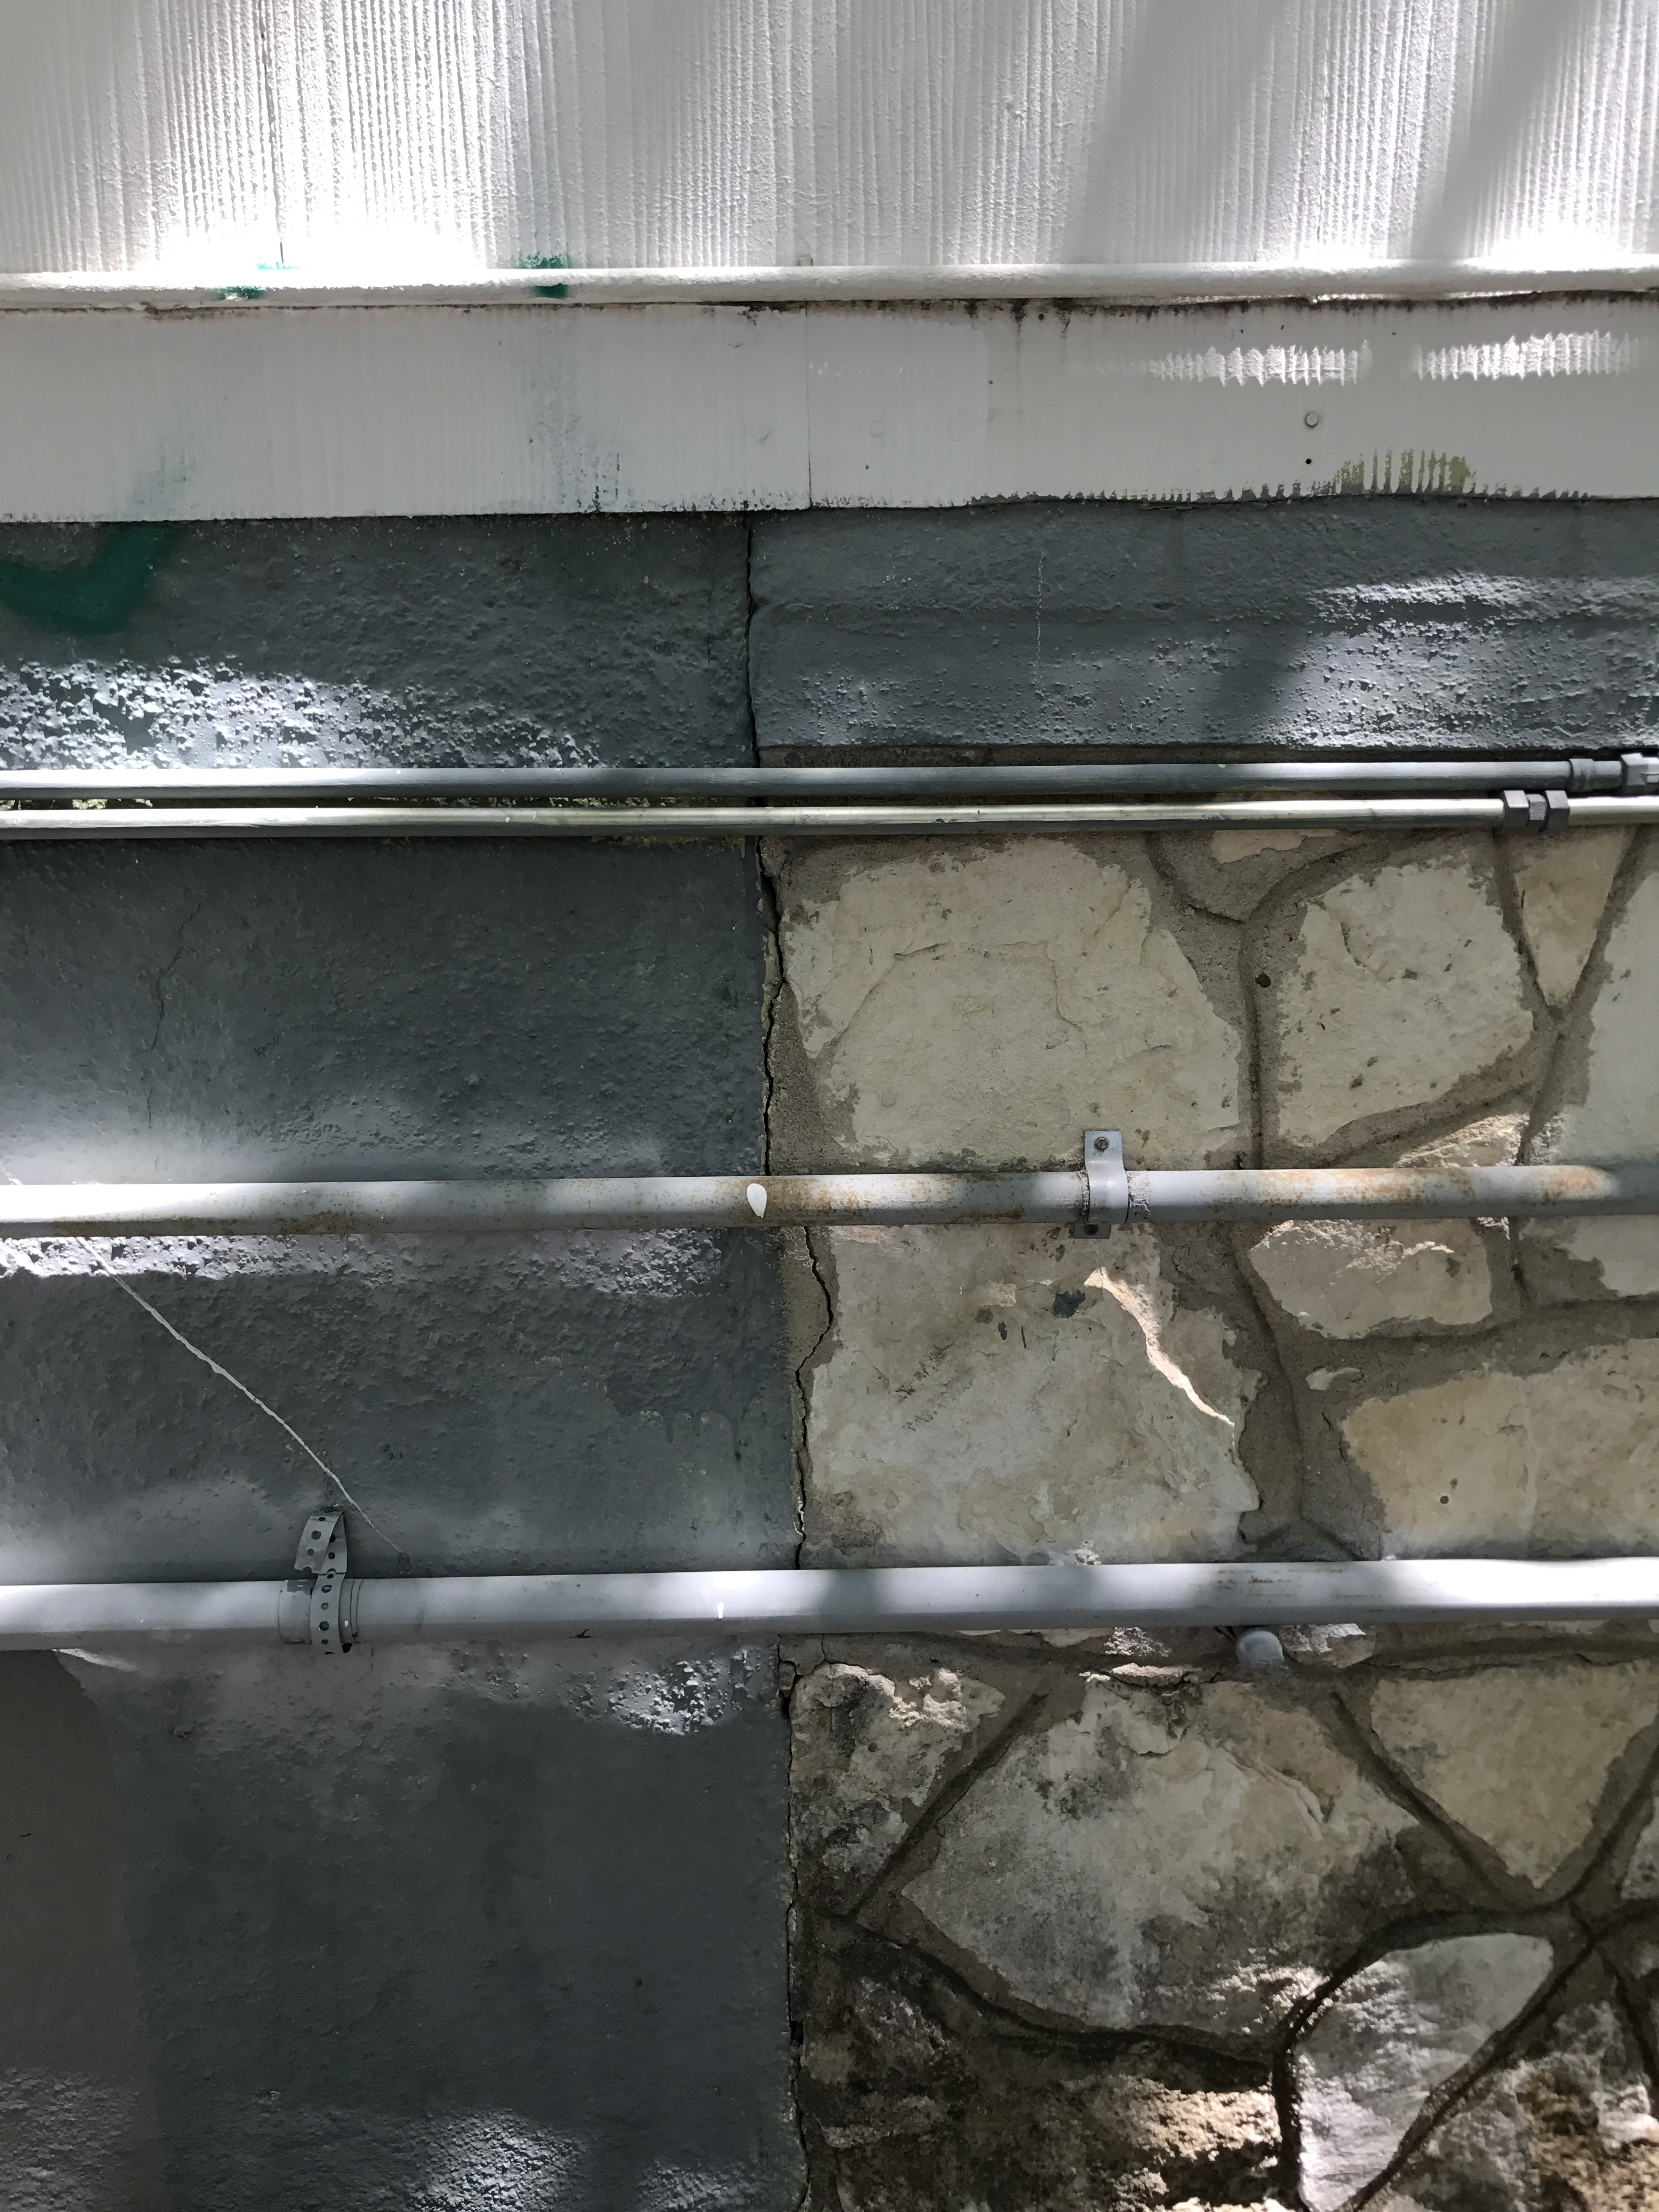
\includegraphics[width=.5\linewidth]{Lindsey_Figure_14}
	\caption{Variation in fabric on west side\\
		{\normalfont\scriptsize \copyright\
			\shortauthor
	}}
	\label{fig:Lindsey_Figure_14}
\end{figure}

If an addition was built, it appears to have been early in the building's history and using rough-cut stone as a foundational element. This change occurs at 56'3.6” (c. \num{17.7} meters) from the front of the building. If this does mark a rear addition, the original floor plan would have been about \num{20} feet (about \num{6} meters) shorter than the current floor plan. The rubble fabric extends past the base of the building for a short distance before turning into stairs which allow access to the backyard and the Cazares’ home through a wooden gate.

Cazares has added quite a few extra shelves to the original ones. Wire racks (which I did not include on the map because of their easy mobility) fill some space that the shelving does not. And in the back room, drums and other musical equipment as well as martial arts gear is somewhat haphazardly placed about. Most are quite mobile, so they're unmapped. The most important changes to the interior of the structure itself are the removal of the ice box and the removal of kitchen equipment in the back. The ice box faced outward along the north wall of the facade so that customers could grab their ice from outside as they left. When the family stopped selling ice it became a storage area for returnable soda bottles, according to Cazares. When they replaced the doors in the late 1980s, Cazares said they blocked up the wall as well.

%FIGURE 15: New shelving
\begin{figure}[!tb]
	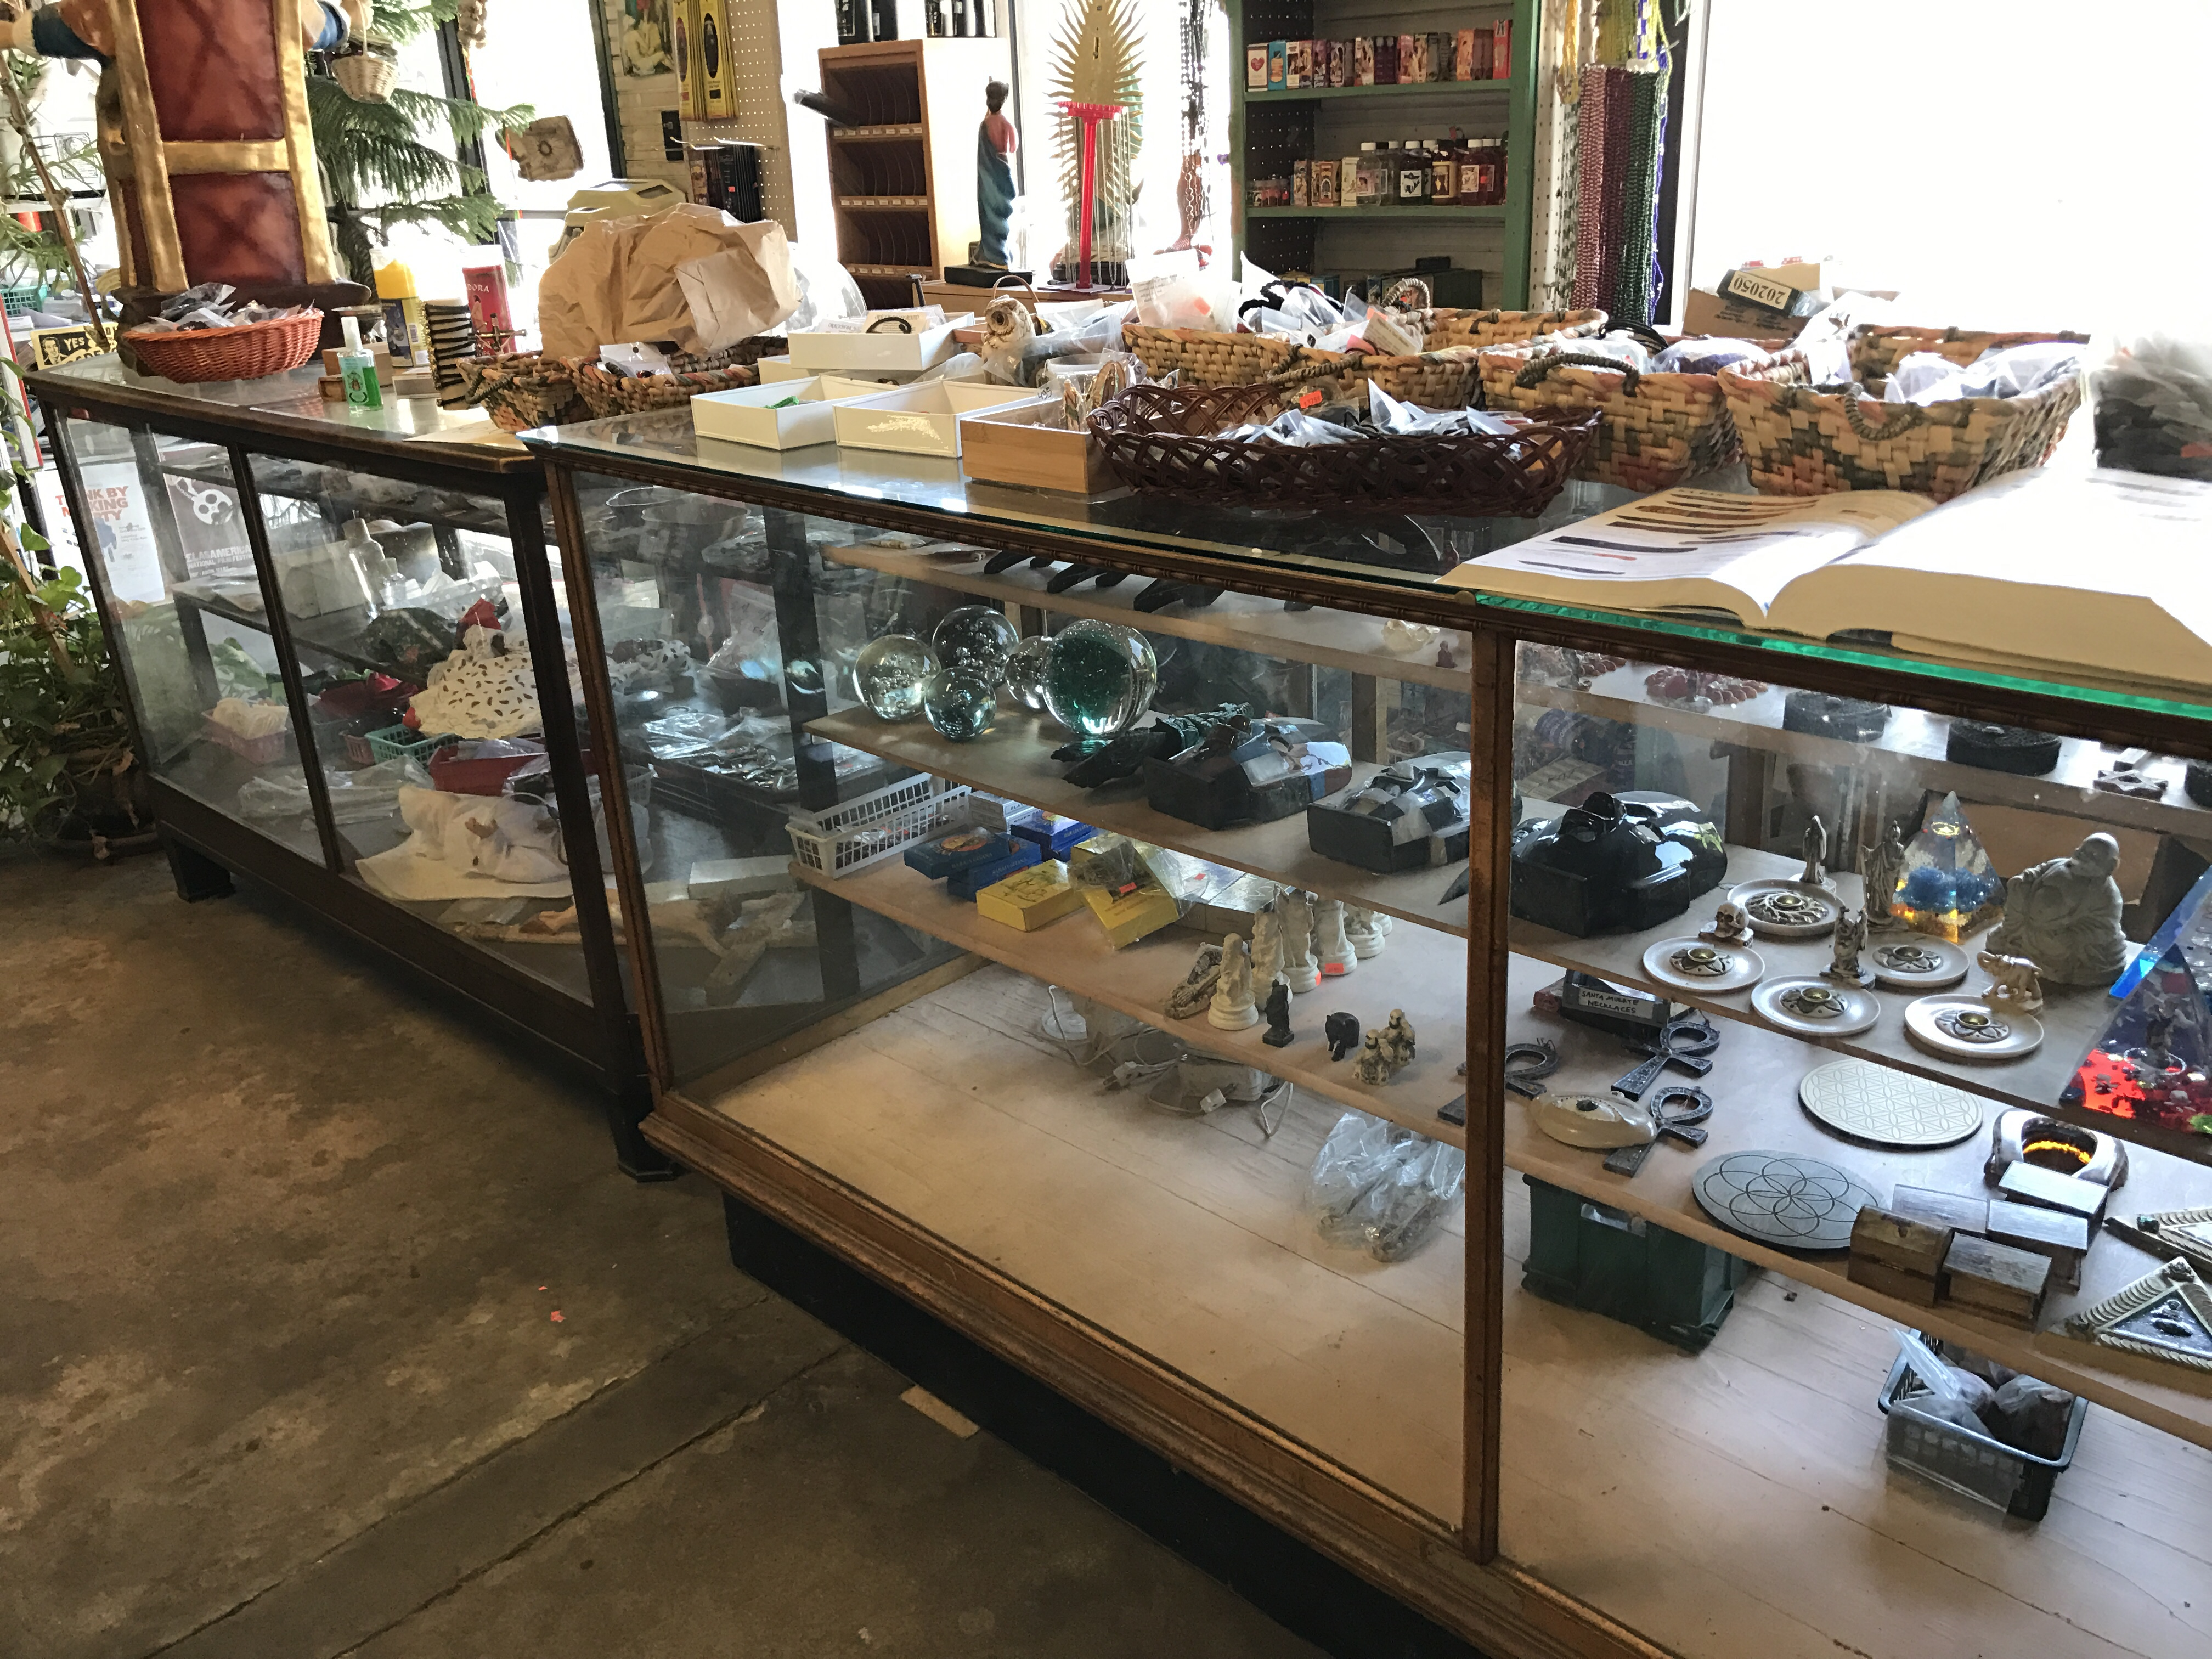
\includegraphics[width=.5\linewidth]{Lindsey_Figure_15}
	\caption{New shelving showcasing Mesoamerican-style stone masks\\
		{\normalfont\scriptsize \copyright\
			\shortauthor
	}}
	\label{fig:Lindsey_Figure_15}
\end{figure}

The kitchen equipment has also been gone for years, but a wall in the back room still includes tiling suggestive of a kitchen space. There are three smaller rooms behind that wall in the southernmost portion of the building, a washroom with a sink, a restroom with a toilet, and a storage area. A door in this area leads out to the lawn and to the house behind the store. While a refrigerator in the area is new, much of the material in this space looks quite old and the wall paneling is similar to that used on other portions of the structure.

%FIGURE 16: Back
\begin{figure}[!tb]
	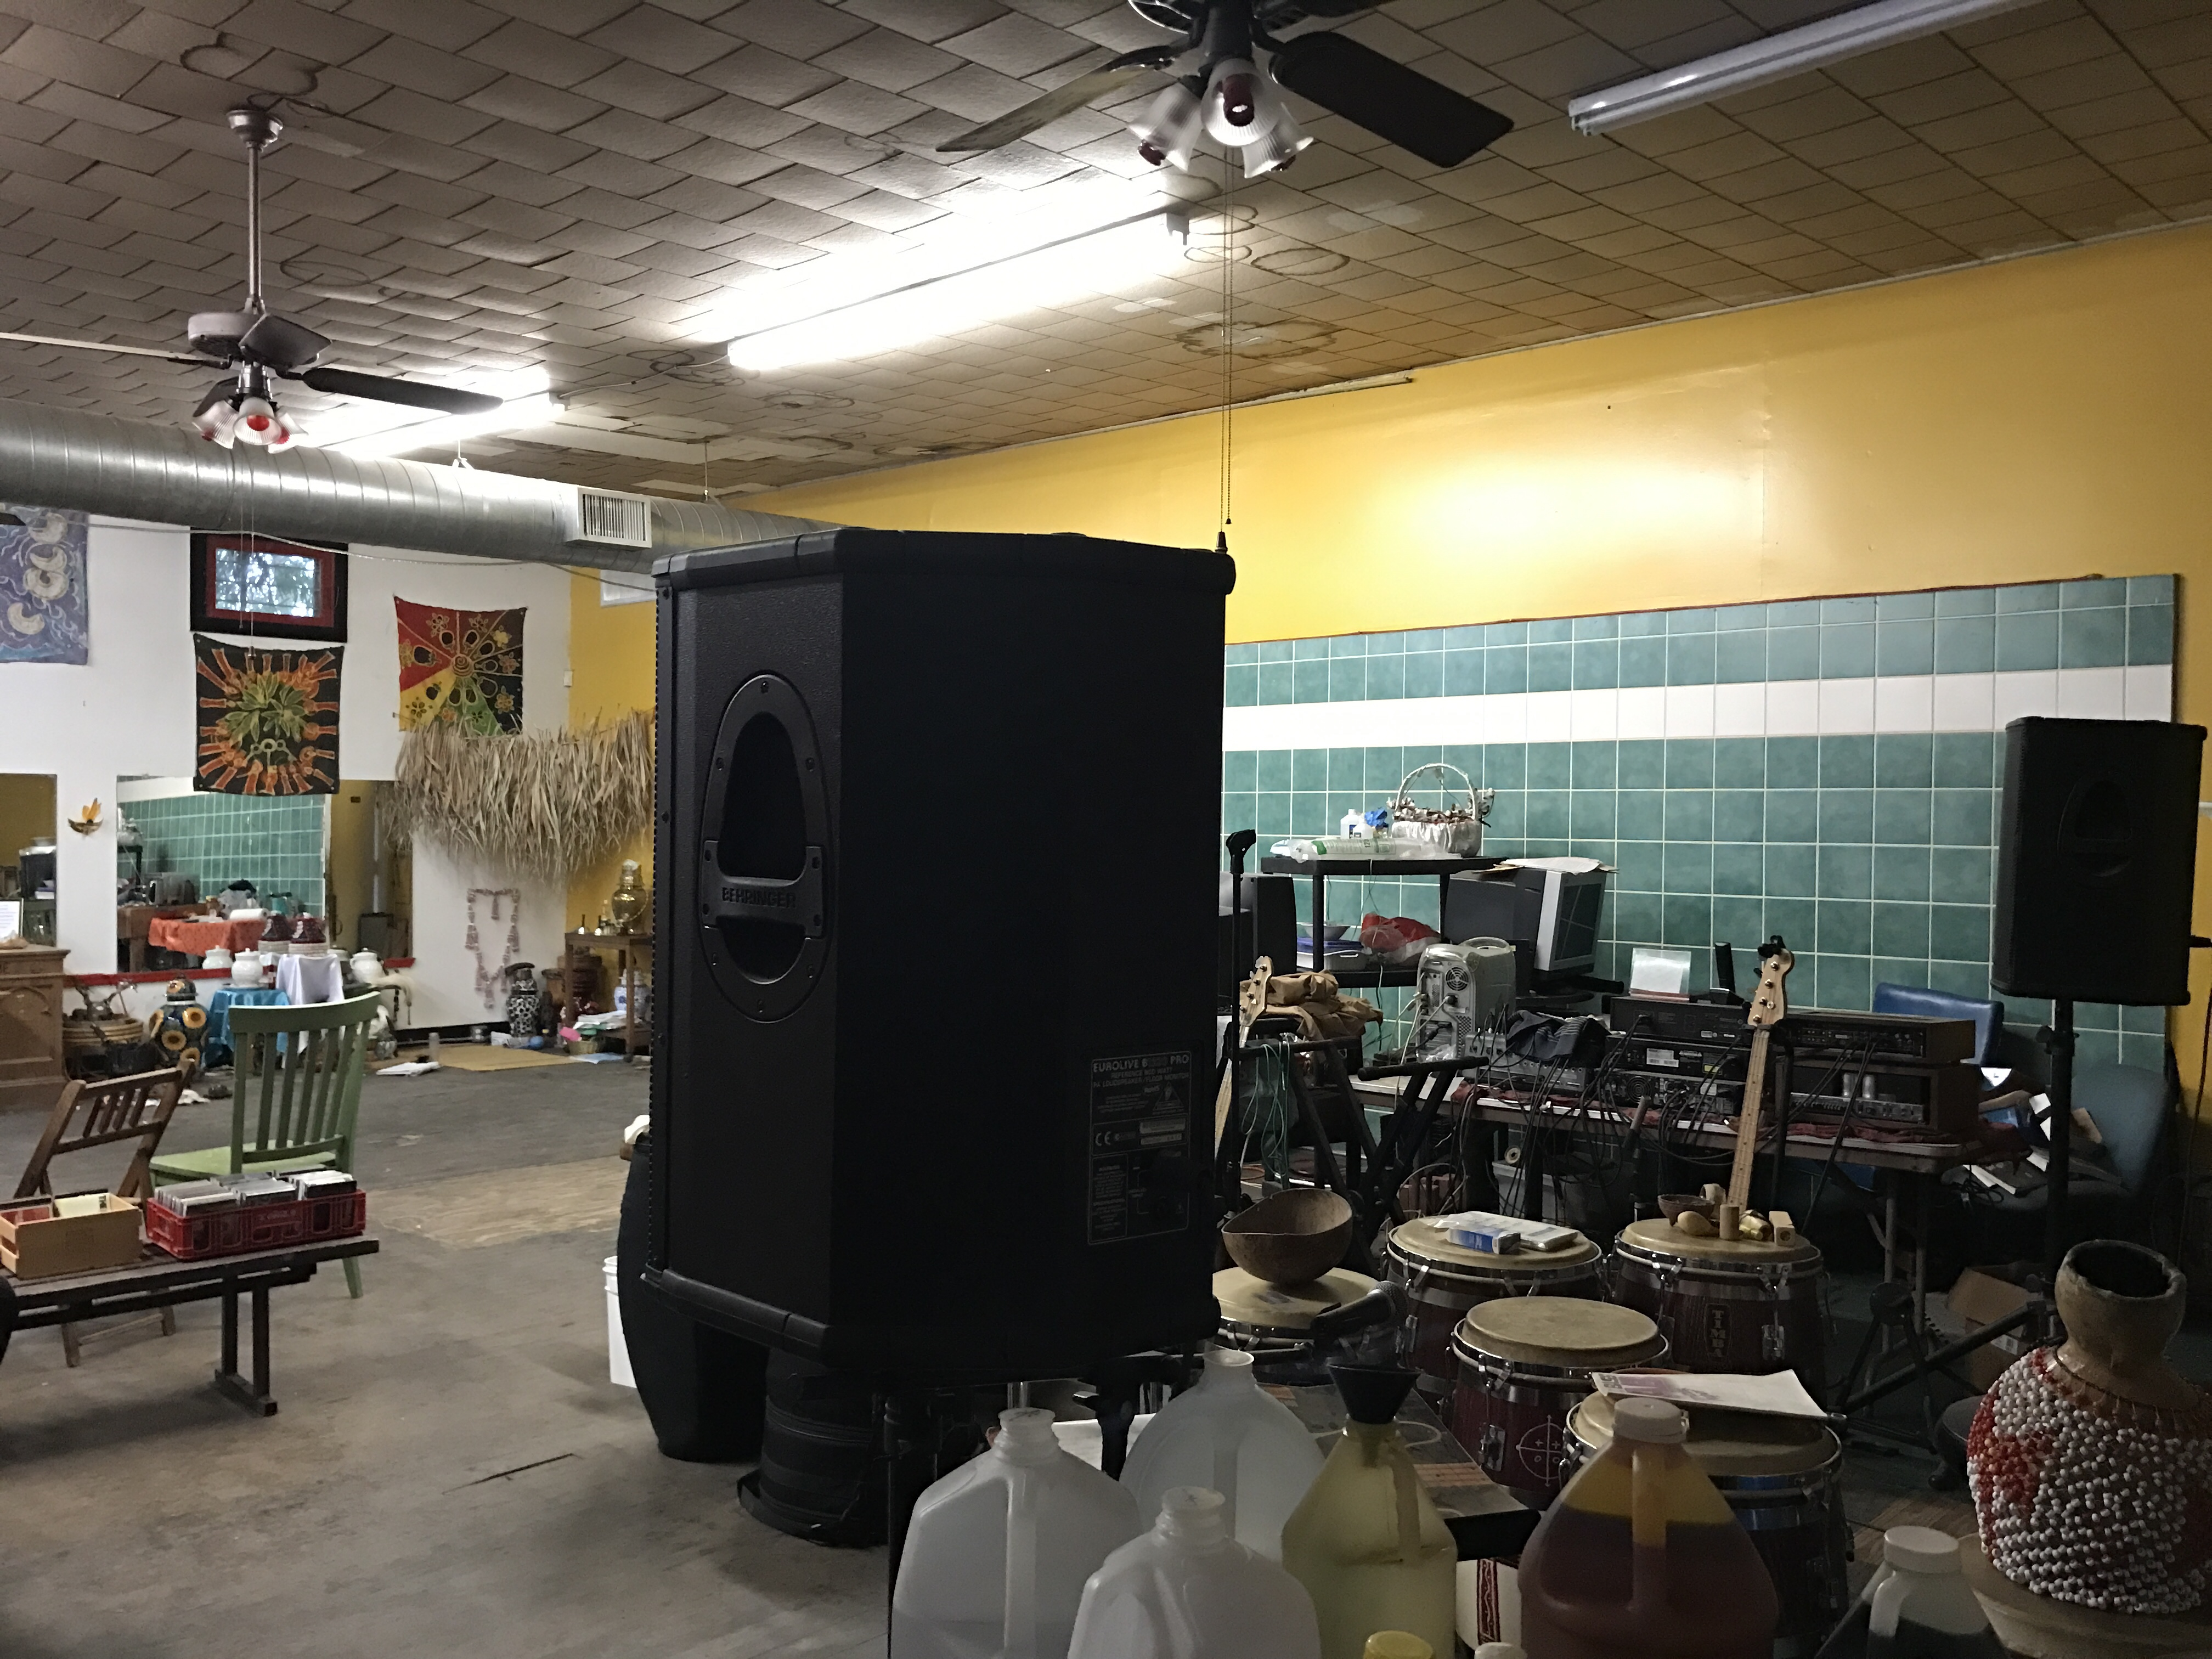
\includegraphics[width=.5\linewidth]{Lindsey_Figure_16}
	\caption{The back room\\
		{\normalfont\scriptsize \copyright\
			\shortauthor
	}}
	\label{fig:Lindsey_Figure_16}
\end{figure}

\IJSRAsection{Contexts of the Green and White Grocery}

Small, locally-owned grocery stores in Indianapolis were most common from the late 19\textsuperscript{th} to early 20\textsuperscript{th} century according to \textcite{mullins}. In the case of African-American grocery stores, the model collapsed in the 1930s due to urban renewal and an increase in chain stores (\cite[88]{mullins}). However, for whatever reason, Austin’s corner stores did not suffer the same fate in the 1930s; whichever of the three building dates is correct, the Green and White Grocery was still a true grocery store in the 1970s. Other important East Austin grocery stores also survived the 1930s. Hardy, Heck, Moore, Inc. (2016) surveyors list seven buildings that hosted grocery stores at some point in East Austin: two were built after the 1930s, four changed uses in the late 1960s or early 1970s. One, the Comal Food Store, operated until at least the early part of 2017. However, as of the writing of this paper, a fence has blocked access to the structure for at least two months. It is unclear if the store will open again or not.


\textcite{mullins} notes the ethnic insularity of many grocery stores in Indianapolis; while he describes African-Americans occasionally creating campaigns to patronizing other African-American businesses, it is hard to imagine a large amount of choice in this insularity. Noberto and Susie Lopez, the original owners of the Green and White Grocery property, also opened their grocery store in a predominantly Mexican-American community and served a predominantly Mexican-American population, but it is difficult to say whether that was choice, opportunity, or the rigid segregation of Austin at the time (\cite{hernandez}).
Noberto and Susie's descendants remember their grandparents as deeply committed to their community like the other store owners described in \textcite{mullins}. The original grocery store provided a service Cazares still provides: credit. He and other family members declare it the first Mexican-American store in Austin to offer credit (\cite{lepe}). While it is probably impossible to verify, a casual search of evidence related to Austin development does not find any other claimants to the title. John even noted something important about his grandparents' perception of clients: in the book Noberto kept listing how much people owed, each customer was listed by name, not a number. This suggests Noberto saw his clients as members of a community, not simply potential sources of profit, according to Cazares.


More importantly, store stocking principles were different. Mullins describes a careful negotiation with Anglo-American goods and African-American cultural preference at the store in Indianapolis with an example: his team found only one African-American-style broach on the property despite the majority African-American store patrons (\cite[92]{mullins}). But Mexican culture was more accessible in Texas than African culture in Indianapolis, and the goods at the Green and White Grocery have always represented that. Cazares does remember selling hamburgers, but he 
(and almost everyone interviewed by \textcite[75-76]{lepe} and \textcite{gandara}) 
also remembers selling tamales, a pre-Hispanic food still eaten in most parts of Mexico. Because of Austin's proximity to Mexico, Noberto was able to travel to Mexico to buy goods like regionally-made salsas, and in many cases Mexican merchants came to Austin. The ability to stock Mexican goods made the Green and White Grocery an important place for Mexican immigrants who missed certain products and tastes and Mexican-Americans who valued their heritage. One of the merchants Noberto bought his inventory from sold not just salsas but saints’ candles and polvos which are the main inventory of the Green and White Grocery today. As the inventory changed, the clientele's relationship with the Green and White Grocery must have changed as well. But one important aspect remains the same: the goods the Green and White Grocery sells allow Mexican-Americans to connect with their cultural heritage in a way they might not otherwise be able to in a predominantly Anglo-American city. You can't get your eggs and milk there, but the present-day botánica plays a similar role to the original Green and White Grocery.

\IJSRAsection{Conclusion}

More studies on the Green and White Grocery itself would determine exact age of additions, and a small test plot on the east side of the building could perhaps uncover evidence of earlier merchandise sold at the store. Also, John and his family live on the property as previous family members did. Their home was built in the late 1940s according to Travis Central Appraisal District records (\cite[75-76]{tcad}). This second building was left out of the survey, but a future survey could examine it. This would allow us to better understand the relationships business owners had with their stores. As living on the same property as a business was also common in Indianapolis (\cite{mullins}), it is important to know if this trend crosses ethnic groups and what these houses commonly looked like.

But perhaps the most pressing study for the East Austin area is one which compares the Green and White Grocery to other minority-owned businesses: how common were trends like living on the property or starting out as food truck vendors? A broader understanding of East Austin history will make it easier to safeguard both individual structures like the Green and White Grocery and the history of East Austin in general. John has a daughter, and she could very well take over the store if she wants, phasing it slowly into something new. But as the property taxes rapidly rise (\cite{tcad}), it is necessary to recognize the property as both important in the historical and contemporary culture of East Austin, or the Green and White Grocery could pass from the hands of the family and disappear the way other important East Austin structures have.

\IJSRAseparator

\IJSRAsection{Acknowledgements}
Thanks to John Cazares for allowing access and for keeping the author supplied with copal; thanks to Erica Matos-Lindsey for assisting with measurement.

\IJSRAclosing%<---- don’t change this!
